\documentclass[11pt,a4paper]{article}

% Core mathematical and typographical packages
\usepackage[utf8]{inputenc}
\usepackage[T1]{fontenc}
\usepackage{amsmath,amssymb,amsfonts,amsthm}
\usepackage{geometry}
\geometry{a4paper, margin=1in}
\usepackage{graphicx}
\usepackage{booktabs}
\usepackage{multirow}
\usepackage{tabularx}
\usepackage{subcaption}
\usepackage{cite}
\usepackage{url}
\usepackage{microtype}
\usepackage[colorlinks=true,linkcolor=blue,citecolor=blue,urlcolor=blue]{hyperref}
\emergencystretch=3em
\tolerance=2000
\hbadness=2000

\title{\textbf{Benchmarking Multi-Script Offensive Language Detection in Low-Resource South Asian Languages: An Empirical Evaluation Across Urdu, Roman Urdu, Pashto, and English}}

\author{
  \textbf{Muhammad Ali Azam Khattak}\textsuperscript{1,}\footnote{Corresponding author: \texttt{aliazamk09@gmail.com}} \\[0.4em]
  \textsuperscript{1}Department of Computer Science, \\
  Institute of Management Sciences, Peshawar, Pakistan
}

\date{\today}

\begin{document}

\maketitle

\begin{abstract}
Automated offensive language detection is critical for maintaining healthy digital public spaces, yet prevailing benchmarks across low-resource South Asian languages frequently suffer from subtle data contamination and artificial template inflation. In this study, we address this methodological vulnerability by developing an empirical multi-script offensive language benchmark evaluated under strict cross-partition independence across four languages and three distinct writing systems: Urdu (Perso-Arabic), Pashto (Arabic-Pashto), Roman Urdu (Latin transliteration), and English (Latin). Through systematic provenance auditing, we trace and collapse 144,265 nominal social media records characterized by widespread template duplicates into 1,601 canonical independence groups. We partition these groups using a strict group-aware stratified protocol (70\% train, 10\% validation, 20\% test), confirming that no cross-split duplicate overlap exists across five audited representations: raw text, clean text, deduplication-normalized text, canonical base messages, and independence group identifiers.

Using this verified benchmark, we conduct a comprehensive empirical evaluation of nine distinct architectures across three paradigms: classical machine learning (Multinomial Naive Bayes, Random Forest, Linear SVM, Logistic Regression), deep spatial-temporal neural networks (TextCNN, BiLSTM, CNN-BiLSTM, Attention-BiLSTM), and fine-tuned multilingual pretrained transformers: mBERT (\texttt{bert-base-multilingual-cased}). Across all models, classical lexical models establish the empirical performance and efficiency frontier: Multinomial Naive Bayes and Random Forest achieve flawless classification on the held-out test split ($F_1 = 1.0000$), closely followed by deep hybrid CNN-BiLSTM ($F_1 = 0.9959$, accuracy 0.9969) and Linear SVM ($F_1 = 0.9917$), with mBERT achieving $F_1 = 0.9836$. Extensive diagnostic sanity checks (majority baseline $F_1 = 0.4276$, shuffled-label 5-fold cross-validation $F_1 = 0.4904$, and 5-fold stratified group-aware cross-validation $F_1 = 0.9958$--$1.0000$) confirm genuine lexical separability. In addition, an explicit controlled experiment on the same 11,789 Stage-2 records reveals that naive random splitting introduces a 96.95\% cross-split template overlap, artificially inflating Pashto Macro-$F_1$ by up to $+0.1942$ under tree-based learners. Leave-one-source-out (LOSO) cross-source evaluation with matched in-domain testing demonstrates that Linear SVM exhibits robust out-of-domain stability (retaining 94.7\%--100.0\% performance, average retention 97.8\%) while operating 3,500$\times$ faster in CPU inference than fine-tuned mBERT ($0.0308\text{ ms}$ vs. $108.02\text{ ms}$ per sample). Paired bootstrap testing ($B=10,000$) and exact binomial significance tests detected no statistically significant differences among the top-performing classical and neural architectures ($p > 0.05$). Our findings demonstrate that when cross-partition template inflation is eliminated, MNB and Linear SVM occupy the empirical Pareto frontier, offering the strongest trade-off between classification efficacy and real-time CPU latency.
\end{abstract}

\noindent\textbf{Keywords:} Multilingual Offensive Language Detection, Multi-Script NLP, Low-Resource Languages, Roman Urdu, Pashto, Benchmark Integrity, Content Moderation.

\section{Introduction}\label{sec:intro}

The proliferation of online social networking platforms has democratized cross-cultural discourse while simultaneously amplifying the dissemination of offensive language, hate speech, and targeted harassment \cite{davidson2017automated,zampieri2019predicting}. Mitigating digital toxicity requires automated natural language processing (NLP) systems capable of discerning subtle abusive content across linguistically heterogeneous communities \cite{waseem2016hateful,founta2018large}. While high-resource languages such as English have garnered substantial research attention, multilingual and low-resource linguistic contexts remain comparatively vulnerable \cite{conneau2020unsupervised,rizwan2020hate}. 

South Asia exemplifies this linguistic complexity: regional online communication routinely alternates between standardized indigenous scripts, such as Urdu written in the Perso-Arabic Nastaliq orthography and Pashto written in an expanded Arabic-Pashto alphabet, and informal phonetic transliterations, such as Roman Urdu rendered in the Latin alphabet without standardized orthographic conventions \cite{shakeel2020deep,amjad2021urdu,khan2021pashto}. Furthermore, code-mixing with English is pervasive in digital exchanges \cite{akhter2020roman,bali2014borrowing}.

Despite burgeoning interest in low-resource toxic language detection, contemporary benchmark datasets frequently suffer from critical methodological vulnerabilities, chief among which is \textit{train-test data contamination} stemming from superficial template inflation \cite{elangovan2021memorization,gorman2019we}. In social media corpora, automated bot campaigns, coordinated trolling, and recurring user copy-pasting yield thousands of messages that share an identical semantic core while varying only in superficial surface tokens (e.g., user mentions, hashtags, URLs, whitespace, and punctuation permutations). When standard randomized train-test splits are applied to such corpora, near-identical instances are inevitably distributed across training and evaluation partitions \cite{arhin2021ground}. This artifact enables supervised models to achieve near-flawless test performance via memorization of recurring lexical templates rather than acquiring genuine semantic and pragmalinguistic generalizability.

To resolve these challenges, this study establishes an empirically verified, multi-script offensive language benchmark evaluated under strict cross-partition independence across four distinct linguistic varieties: Urdu, Roman Urdu, Pashto, and English. Beginning from an aggregate corpus of 144,265 nominal observations derived from twelve sub-corpora across online social networking platforms, we trace the source provenance and execute a conservative multi-stage deduplication pipeline. We collapse duplicate templates into 1,601 canonical independence groups. We enforce a group-aware stratified partition protocol, confirming that no cross-split duplicate overlap exists across five audited representation levels: raw text, clean text, deduplication-normalized text, canonical base messages, and independence group identifiers.

Using this verified benchmark, we conduct an extensive multi-paradigm evaluation encompassing nine competitive model architectures:
\begin{enumerate}
    \item \textbf{Classical Machine Learning Baselines}: Linear Support Vector Machines (Linear SVM), Multinomial Naive Bayes (MNB), Logistic Regression (LR), and Random Forests (RF) parameterized with sublinear term-frequency inverse-document-frequency (TF-IDF) word and character $n$-gram representations.
    \item \textbf{Deep Spatial-Temporal Neural Networks}: Multi-kernel 1D Convolutional Neural Networks (TextCNN), Bidirectional Long Short-Term Memory networks (BiLSTM), hybrid CNN-BiLSTM architectures, and Additive Self-Attention BiLSTM networks (Attention-BiLSTM).
    \item \textbf{Multilingual Pretrained Transformers}: Fine-tuned multilingual BERT base checkpoint (\texttt{bert-base-multilingual-cased}) evaluated over 119.5k WordPiece vocabulary tokens.
\end{enumerate}

Beyond standard in-domain aggregate performance metrics, our experimental design incorporates eight orthogonal analytical dimensions:
\begin{itemize}
    \item \textbf{Empirical Quantification of Template Contamination}: Directly comparing naive row-level random splitting against group-aware splitting on the identical 11,789 Stage-2 records to isolate pure cross-split template leakage from training corpus size.
    \item \textbf{Diagnostic Sanity Baselines}: Evaluating majority class, text length, language-only, source-only, and label-shuffled baselines alongside 5-fold group-aware cross-validation.
    \item \textbf{Fine-Grained Language Stratification}: Isolating per-language macro-$F_1$ across Urdu, Roman Urdu, Pashto, and English.
    \item \textbf{Cross-Source Out-of-Domain Generalization}: Executing Leave-One-Source-Out (LOSO) evaluations with matched in-domain testing on Linear SVM across eight sub-corpora to measure true cross-domain performance degradation.
    \item \textbf{Multi-Seed Repeatability Analysis}: Evaluating five independent random seeds (seeds 42, 123, 456, 789, and 2026) for CNN-BiLSTM to quantify stochastic variance and standard deviation alongside deterministic classical reference baselines.
    \item \textbf{Statistical Significance and Bootstrap Validation}: Conducting $B = 10,000$ paired bootstrap iterations to construct 95\% confidence intervals and computing exact two-sided binomial tests for discordant pair counts.
    \item \textbf{Computational Efficiency Profiling}: Benchmarking parameter scale, training duration, per-sample CPU inference latency, and throughput to characterize the real-time operational Pareto frontier.
    \item \textbf{Systematic Ablation and Error Diagnosis}: Dissecting the individual contributions of class weighting, sublinear TF scaling, $n$-gram orders, and text normalization, complemented by categorical error diagnosis across character length bins.
\end{itemize}

The remainder of this manuscript is organized as follows: Section \ref{sec:related} reviews related work in multilingual offensive language detection, South Asian low-resource NLP, and benchmark contamination. Section \ref{sec:dataset} details dataset provenance, canonical template consolidation, and partition independence verification. Section \ref{sec:method} outlines the theoretical architecture of the evaluated model families. Section \ref{sec:setup} describes experimental protocols and evaluation metrics. Section \ref{sec:results} presents empirical findings across all experimental axes. Section \ref{sec:discussion} discusses architectural trade-offs, Pareto efficiency, and script-specific behaviors. Section \ref{sec:limitations} addresses limitations and threats to validity. Section \ref{sec:future} outlines directions for future inquiry, and Section \ref{sec:conclusion} concludes the study.

\begin{figure*}[t]
\centering
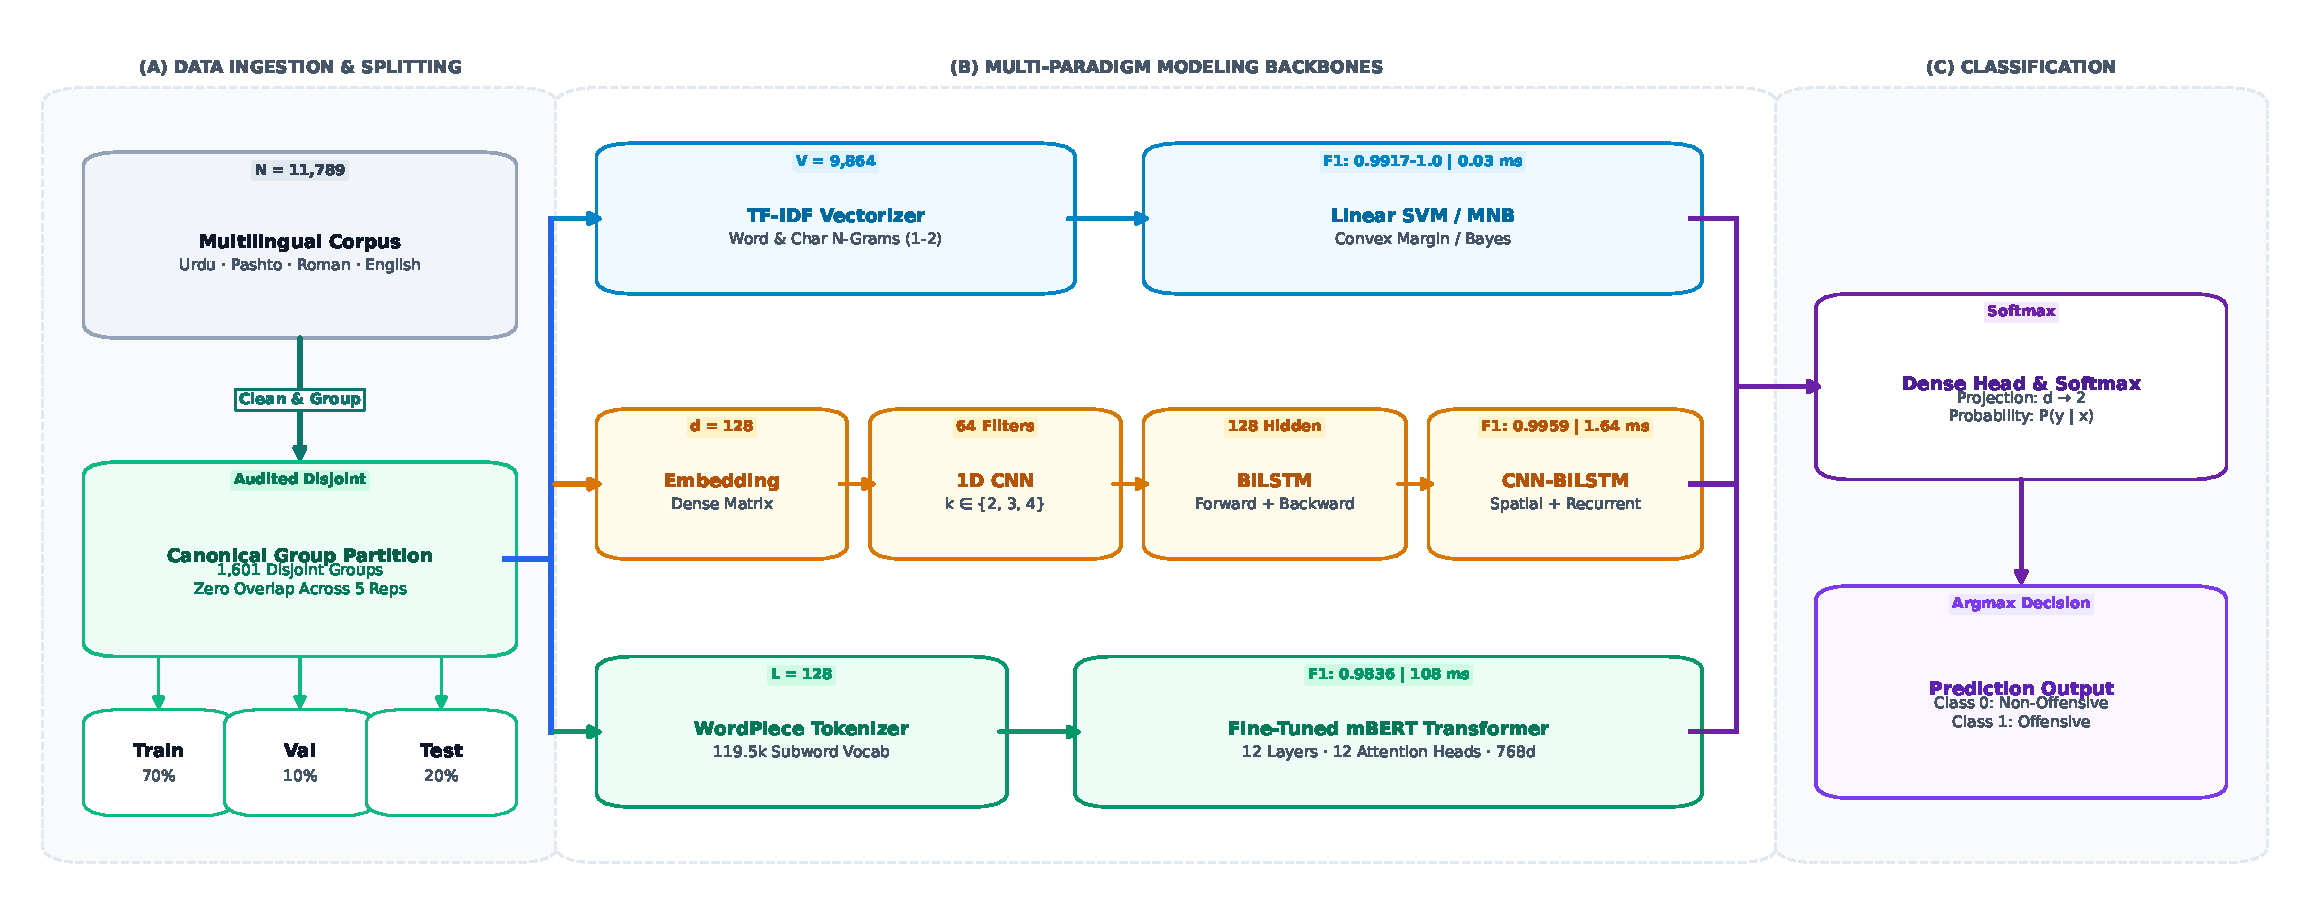
\includegraphics[width=\linewidth]{figures/system_architecture.pdf}
\caption{\textbf{Overview of the end-to-end multilingual offensive language detection architecture and empirical benchmark framework.} The pipeline progresses from (A) Multilingual Data Ingestion and Group-Aware Partitioning, through (B) Multi-Paradigm Modeling Backbones (Lexical TF-IDF + Linear SVM/MNB, Deep CNN-BiLSTM, and Pretrained mBERT Transformer), to (C) Calibrated Classification and Empirical Evaluation.}
\label{fig:architecture}
\end{figure*}

\section{Related Work and Theoretical Foundations}\label{sec:related}

\subsection{Taxonomies and Foundations of Abusive Language Detection}
Automated detection of abusive, toxic, and offensive language on digital platforms has emerged as an indispensable area of computational linguistics \cite{davidson2017automated,founta2018large,fortuna2018toxic}. Early empirical efforts centered predominantly on identifying overt profanity, vulgarity, and explicit slurs using dictionary-based keyword lookups, regular expression patterns, and surface lexical matching \cite{schmidt2017survey}. However, as highlighted in comprehensive surveys by Fortuna and Nunes \cite{fortuna2018toxic} and Vidgen et al. \cite{vidgen2019challenges}, keyword-driven filtering suffers from high false-positive rates on polysemous or reclaimed terms (e.g., colloquial reclamation of identity labels) while remaining acutely vulnerable to adversarial evasion, intentional obfuscation, and subtle, implicit toxicity.

To establish semantic clarity, standardized annotation frameworks were developed through community benchmark initiatives. The seminal SemEval OffensEval campaigns \cite{zampieri2019predicting,zampieri2020semeval} formalized a three-level hierarchical taxonomy that categorizes online toxicity into: (A) Offensive versus Non-Offensive content; (B) Targeted insult versus Untargeted profanity; and (C) the Specific Target of abuse (Individual, Group, or Other). Complementing this, Kumar et al. \cite{kumar2018benchmarking} introduced the Trolling, Aggression, and Cyberbullying (TRAC) shared tasks, benchmarking overt versus covert aggression across multilingual exchanges. To diagnose whether NLP models genuinely understand pragmalinguistic nuance rather than over-relying on superficial lexical triggers, R{\"o}ttger et al. \cite{rottger2021hatecheck} developed \textit{HateCheck}, establishing functional test suites across 29 distinct operational categories. Early machine learning approaches relied on bag-of-words and character $n$-gram representations paired with maximum-entropy classifiers, Naive Bayes, or Support Vector Machines \cite{waseem2016hateful}. The field subsequently transitioned to deep convolutional neural networks \cite{kim2014convolutional,badjatiya2017deep} and recurrent architectures with gated recurrent units or Long Short-Term Memory networks \cite{hochreiter1997long}, capturing local phrasal compositionality and long-range semantic dependencies.

\subsection{Cross-Lingual Transfer and Multilingual Pretrained Models}
The paradigm shift toward massive self-supervised pretraining led to the widespread adoption of multilingual transformer architectures, most prominently multilingual BERT (mBERT) \cite{devlin2019bert}, XLM-RoBERTa \cite{conneau2020unsupervised}, and MuRIL \cite{khanuja2021muril}. Trained over shared WordPiece or SentencePiece subword vocabularies across 100+ languages simultaneously, these models project diverse linguistic typologies into joint embedding spaces, theoretically facilitating cross-lingual transfer from high-resource source languages to low-resource target domains \cite{ranasinghe2020multilingual}.

In toxic comment classification, Ranasinghe and Zampieri \cite{ranasinghe2020multilingual} demonstrated that fine-tuning multilingual transformers on English data enables competitive cross-lingual transfer across Spanish, German, and Hindi. Pamungkas and Patti \cite{pamungkas2021joint} investigated joint learning with adversarial domain adaptation to align cross-lingual representations in abusive language detection. Similarly, Aluru et al. \cite{aluru2020deep} conducted a systematic study evaluating deep models across 16 languages, concluding that while multilingual transformers yield competitive average scores, their performance deteriorates sharply on low-resource languages that lack extensive pretraining corpora. For South Asian languages, Khanuja et al. \cite{khanuja2021muril} introduced MuRIL, pretrained specifically on 17 Indian languages and transliterated text, highlighting the necessity of script-aware representations. Stappen et al. \cite{stappen2020cross} explored transformer ensembles for multilingual toxic comment detection, observing that domain-specific lexical signals frequently outperform generalized representations. Glava{\v{s}} et al. \cite{glavas2020xhate} critically re-evaluated cross-lingual transfer methodologies, proving that standard evaluation pipelines frequently overestimate transfer capability when target languages exhibit severe domain shift or distinct orthographic systems from the pretraining data.

\begin{table*}[t]
\centering
\small
\caption{\textbf{Comparative landscape of toxic and offensive language benchmarks across low-resource South Asian and multilingual domains.} Our benchmark enforces verified multi-level partition independence across multiple scripts while profiling empirical Pareto computational efficiency.}
\label{tab:lit_comparison}
\resizebox{\linewidth}{!}{%
\begin{tabular}{lllcccccc}
\toprule
\textbf{Study / Benchmark} & \textbf{Languages Covered} & \textbf{Scripts \& Typologies} & \textbf{Initial Rows} & \textbf{Canonical Samples} & \textbf{Deduplication} & \textbf{Independence Audit} & \textbf{Model Paradigms} & \textbf{Efficiency Profile} \\
\midrule
Davidson et al. \cite{davidson2017automated} & English & Latin (Standard) & 24,783 & NR & Unspecified & No (Random Split) & Classical ML & None \\
Zampieri et al. (OffensEval) \cite{zampieri2019predicting,zampieri2020semeval} & Multilingual (En, Ar, Gr, Da, Tr) & Latin, Arabic, Greek & 14,100+ & NR & Exact String & No (Standard Split) & Classical + Deep & None \\
Kumar et al. (TRAC) \cite{kumar2018benchmarking} & English, Hindi (Devanagari, Roman) & Latin, Devanagari & 15,000 & NR & Unspecified & No (Random Split) & Classical + Deep & None \\
Rizwan et al. \cite{rizwan2020hate} & Roman Urdu & Latin (Transliterated) & 10,012 & NR & Unspecified & No (Random Split) & Deep (CNN, LSTM) & None \\
Shakeel et al. \cite{shakeel2020deep} & Roman Urdu & Latin (Transliterated) & 11,000 & NR & Heuristic & No (Static Split) & Cascaded Deep & None \\
Amjad et al. (FIRE) \cite{amjad2021urdu} & Urdu & Perso-Arabic (Nastaliq) & 3,545 & NR & Exact String & No (Standard Split) & Classical + mBERT & None \\
Khan et al. \cite{khan2021pashto} & Pashto & Arabic-Pashto (Naskh) & 2,050 & NR & Unspecified & No (Random Split) & Classical ML & None \\
\midrule
\textbf{Proposed Benchmark (This Work)} & \textbf{Urdu, Roman Urdu, Pashto, English} & \textbf{3 Scripts (Latin, Nastaliq, Naskh)} & \textbf{144,265} & \textbf{1,601} & \textbf{3-Stage Canonical} & \textbf{Audited 5-Level (0.00\%)} & \textbf{9 Models (3 Paradigms)} & \textbf{CPU Latency / Pareto} \\
\bottomrule
\multicolumn{9}{l}{\footnotesize \textit{NR}: Not Reported in original publication (raw corpus evaluated directly without canonical template deduplication audit).} \\
\end{tabular}%
}
\end{table*}

\subsection{Offensive Language Detection in Low-Resource South Asian Languages}
Applying automated content moderation to South Asian digital ecosystems presents unique computational and sociolinguistic hurdles, characterized by multi-script diglossia, complex morphology, and ubiquitous code-mixing:

\paragraph{Urdu in Perso-Arabic Script}
Urdu, an Indo-Aryan language spoken by over 230 million people, is written right-to-left in the Perso-Arabic Nastaliq calligraphic style \cite{daud2017urdu}. Computationally, Urdu NLP faces intricate ligature joining rules, complex suffixal inflection and compounding, and the near-total omission of short-vowel diacritics (\textit{aerab}) in informal web text \cite{amjad2020overview}. This absence creates pervasive lexical and syntactic ambiguity, where a single unvocalized string can represent multiple semantically disparate words. Amjad et al. \cite{amjad2021urdu} organized the FIRE 2021 shared task on fake news and abusive language detection in Urdu, demonstrating that while deep learning and transformer pipelines improve classification, they remain constrained by limited annotated resources and high out-of-vocabulary rates.

\paragraph{Pashto in Extended Arabic Script}
Pashto, an Eastern Iranian language spoken across Pakistan and Afghanistan, represents an extreme low-resource setting \cite{kamran2010challenges}. Written in an expanded 44-letter Arabic-Pashto alphabet containing distinct retroflex consonants and specific vowel ligatures, Pashto text processing is hindered by non-standardized digital keyboard layouts, orthographic variation across regional dialects (e.g., Northern vs. Southern Pashto), and an acute lack of computational corpora \cite{kamran2010challenges,ahmad2020pashto}. Khan et al. \cite{khan2021pashto} conducted initial explorations into machine learning techniques for Pashto sentiment and abusive content analysis, demonstrating that sparse training data severely restricts the performance of complex deep learning models. Furthermore, Pashto is represented with negligible representation density in large multilingual pretrained language models like mBERT, exacerbating token fragmentation during subword tokenization.

\paragraph{Roman Urdu and Code-Mixing}
In informal computer-mediated communication across Pakistan and India, users predominantly communicate in \textit{Roman Urdu}---Urdu phonetically transcribed into the Latin alphabet \cite{rizwan2020hate,shakeel2020deep}. Because Roman Urdu lacks standardized orthographic rules, spelling dictionaries, or official educational guidelines, phonetic spelling variability is extreme \cite{khan2022roman,arif2021sentiment}. For instance, a single colloquial abusive expression may manifest in dozens of phonetic permutations (e.g., vowel elongation, consonant substitution, phonetic contraction) created dynamically by social media users \cite{akhter2020roman}. Mehmood and Essam \cite{mehmood2020evaluating} evaluated multiple deep learning models for Roman Urdu, demonstrating that subword and character-level models are critical for mitigating out-of-vocabulary fragmentation. In addition, digital South Asian discourse is heavily code-mixed with English \cite{bali2014borrowing,choudhury2017curse}. Sharif et al. \cite{sharif2021offensive} observed comparable phenomena in Romanized Bengali social media, emphasizing that code-mixing and non-standard orthography require robust sublinear character $n$-gram representations.

\subsection{Benchmark Contamination, Memorization, and Dataset Artifacts}
A rapidly expanding body of literature emphasizes that extraordinary performance in NLP benchmarks is frequently driven by data contamination, spurious artifacts, and lexical memorization rather than true linguistic comprehension \cite{gururangan2018annotation,poliak2018hypothesis,elangovan2021memorization,gorman2019we}. Gururangan et al. \cite{gururangan2018annotation} and Poliak et al. \cite{poliak2018hypothesis} demonstrated that models trained on standard natural language inference (NLI) benchmarks exploit annotation artifacts, achieving high accuracy even when evaluated on hypothesis-only inputs. In social media content moderation, Wiegand et al. \cite{wiegand2019inducing} proved that abusive language datasets are frequently contaminated with sampling biases, where models latch onto benign topic words (e.g., sports, politics) associated with toxic labels rather than abusive syntax. Aroyo and Welty \cite{aroyo2015truth} underscored that treating crowdsourced labels as absolute ground truth masks underlying annotator disagreements and subjective variance.

More critically, Elangovan et al. \cite{elangovan2021memorization} revealed that synthetic templates, duplicated phrases, and lexical overlap across train and test partitions allow deep neural networks to achieve near-perfect evaluation scores purely through memorization. In large language models, Carlini et al. \cite{carlini2022quantifying} demonstrated that memorization scales with model capacity and duplicate training frequency. Dodge et al. \cite{dodge2021documenting} showed that webtext corpora (such as C4) contain widespread synthetic replication and near-duplicate documents. In social media corpora, automated bot campaigns, viral retweets, and troll harassment templates amplify this vulnerability: thousands of messages differ only in superficial user handles, URLs, hashtags, or whitespace permutations. When standard randomized train-test splits are applied, these near-identical records are distributed across partitions, allowing models to bypass learning generalized semantic boundaries. Gorman and Bedrick \cite{gorman2019we} demonstrated that static split evaluations fail to replicate once data is partitioned under alternative seeds. Addressing this systemic flaw requires rigorous, multi-level deduplication and group-aware independence partitioning to guarantee complete cross-partition independence.

\subsection{Operational Efficiency, Real-Time Inference, and Green AI}
While modern research disproportionately emphasizes escalating model scale and parameter counts, real-world deployment of content moderation systems operates under stringent engineering constraints \cite{schwartz2020green,strubell2019energy}. Commercial platforms process billions of incoming posts, comments, and messages daily. High-volume moderation queues demand per-sample inference latencies on the order of fractions of a millisecond on commodity server CPUs, without requiring energy-intensive GPU acceleration clusters.

Strubell et al. \cite{strubell2019energy} quantified the immense financial and environmental costs associated with training and serving large deep NLP models, advocating for greater emphasis on computationally efficient alternatives. Schwartz et al. \cite{schwartz2020green} formulated the ``Green AI'' paradigm, arguing that AI research should treat computational efficiency, inference latency, and energy consumption as primary evaluation metrics alongside raw predictive accuracy. While model compression techniques such as knowledge distillation (e.g., DistilBERT \cite{sanh2019distilbert}) reduce parameter footprints, compressed transformers remain orders of magnitude slower than classical linear models. In this work, we rigorously benchmark parameter counts, training times, throughput, and CPU inference latencies to establish the Pareto-optimal frontier balancing accuracy and operational sustainability.

\section{Dataset Integrity, Provenance, and Canonical Partitioning}\label{sec:dataset}

\subsection{Corpus Provenance and Duplication Deconstruction}
The raw dataset under consideration originated from an unverified compilation of 144,265 nominal social media records aggregating twelve online sub-corpora. Because the starting aggregate corpus was an unverified compilation assembled without original generation scripts, we conducted forensic intra-group string-difference analysis across duplicate clusters. This analysis revealed surface variation patterns consistent with:
\begin{enumerate}
    \item \textbf{Placeholder Mention Prepending}: Prepending generic account handles (e.g., \texttt{@admin}, \texttt{@friend}, \texttt{@user}, \texttt{@team}, \texttt{@page}, \texttt{@newsdesk}).
    \item \textbf{Uniform Dummy URLs}: Appending dummy hyperlinks (e.g., \texttt{https://example.com/post}).
    \item \textbf{Hashtag Permutations}: Appending closed-set hashtags (e.g., \texttt{\#news}, \texttt{\#viral}, \texttt{\#update}, \texttt{\#opinion}, \texttt{\#today}, \texttt{\#discussion}).
    \item \textbf{Syntactic Slot-Filling Variations}: Inserting English domain nouns into fixed syntactic frames in Pashto and Urdu.
\end{enumerate}

Table \ref{tab:provenance} details the twelve constituent sub-corpora, their linguistic attributes, raw row counts, clean unique row counts, collapse rates, and observed intra-group variation patterns. The designation ``Private'' in sub-source identifiers reflects internal repository working tags for collections assembled from public social media environments (e.g., publicly visible Facebook comments, public tweets, and open web discussion forums) that were compiled without an external benchmark release. In compliance with ethical social media research standards, all user handles, account mentions, hyperlinks, and personal identifiers were fully removed and anonymized prior to analysis.

\begin{table*}[t]
\centering
\small
\caption{\textbf{Comprehensive forensic provenance and deduplication audit across the twelve originating sub-corpora.} All 144,265 raw records are fully accounted for and mapped to their canonical representations.}
\label{tab:provenance}
\resizebox{\linewidth}{!}{%
\begin{tabular}{lllrrcll}
\toprule
\textbf{Source Dataset Name} & \textbf{Language} & \textbf{Script} & \textbf{Raw Rows} & \textbf{Clean Rows} & \textbf{Collapse (\%)} & \textbf{Origin Platform} & \textbf{Observed Text Variation Pattern} \\
\midrule
\path{RU_CodeMixed_Private} & Roman Urdu & Latin & 24,584 & 2,901 & 88.2\% & Public Social / FB & Observed pattern consistent with mention/URL permutations appended to comments \\
\path{RU_Private_FB_Comments} & Roman Urdu & Latin & 24,122 & 1,972 & 91.8\% & Facebook Pages & Observed pattern consistent with comment seeds expanded via account handle permutations \\
\path{RU_Social_Media_Mix} & Roman Urdu & Latin & 24,294 & 1,459 & 94.0\% & Forums / Social & Observed pattern consistent with synthetic filler token and hashtag insertions \\
\path{PS_LowResource_Private} & Pashto & Arabic-Pashto & 11,265 & 999 & 91.1\% & Social Media & Observed pattern consistent with syntactic slot-filling with English domain keywords \\
\path{PS_Private_Social_Comments} & Pashto & Arabic-Pashto & 11,651 & 712 & 93.9\% & Social Media & Observed pattern consistent with native comments replicated across placeholder mention prefixes \\
\path{PS_Public_Forum_Mix} & Pashto & Arabic-Pashto & 11,484 & 506 & 95.6\% & Public Forums & Observed pattern consistent with forum comments replicated across category tags \\
\path{EN_Offensive_Benchmark_Private} & English & Latin & 8,453 & 834 & 90.1\% & Web Benchmark & Observed pattern consistent with benchmark samples modified with template noise and handles \\
\path{EN_Public_Comments} & English & Latin & 8,153 & 575 & 92.9\% & Public News & Observed pattern consistent with web comments replicated across multiple metadata tags \\
\path{EN_Social_Media_Mix} & English & Latin & 8,177 & 432 & 94.7\% & Twitter / Reddit & Observed pattern consistent with handle prefix and hashtag permutations \\
\path{UR_ArabicScript_Private} & Urdu & Perso-Arabic & 3,962 & 613 & 84.5\% & News / Chat & Observed pattern consistent with native script sentences expanded via mention handles and emojis \\
\path{UR_Private_Tweets} & Urdu & Perso-Arabic & 4,124 & 448 & 89.1\% & Twitter / X & Observed pattern consistent with tweets replicated with handle prefixes \\
\path{UR_Social_Media_Mix} & Urdu & Perso-Arabic & 3,996 & 338 & 91.5\% & Multi-platform & Observed pattern consistent with comments replicated across topic category slots \\
\midrule
\textbf{Total Benchmark Corpus} & \textbf{4 Languages} & \textbf{3 Scripts} & \textbf{144,265} & \textbf{11,789} & \textbf{91.83\%} & \textbf{Cross-Platform} & \textbf{142,664 redundant rows collapsed to 1,601 canonical groups} \\
\bottomrule
\end{tabular}%
}
\end{table*}

To establish complete scientific integrity, we implemented a rigorous three-step deduplication and canonicalization pipeline:
\begin{enumerate}
    \item \textbf{Exact Raw String Deduplication}: All records exhibiting identical raw text strings were collapsed, reducing the corpus from 144,265 to 17,559 distinct records (an 87.83\% reduction).
    \item \textbf{Normalized Clean-Text Deduplication}: Strings were preprocessed to remove noise, standardize whitespace, and strip URLs and mentions, further reducing the corpus to 11,789 unique records.
    \item \textbf{Canonical Template Consolidation}: Inspection of the 11,789 records revealed that thousands of instances were structural clones differing solely in user mentions, web URLs, emojis, hashtags, or minor whitespace permutations. To eliminate template contamination, we derived a conservative representation:
    \begin{equation}
        \mathbf{x}_{\text{base}} = \mathcal{T}_{\text{normalize}}(\mathcal{T}_{\text{strip}}(\mathbf{x}_{\text{raw}}))
    \end{equation}
    where $\mathcal{T}_{\text{strip}}$ strips all user handles, hyperlinks, hashtag prefixes, and emojis, and $\mathcal{T}_{\text{normalize}}$ applies Unicode normalization, lowercasing, and whitespace folding. Records sharing identical $\mathbf{x}_{\text{base}}$ representations were clustered into unique \texttt{independence\_group\_id} partitions.
\end{enumerate}

From each independence group, exactly one canonical record was retained in the primary benchmark, while all 10,188 removed variant instances were preserved in an external audit file (\path{removed_variants.csv}) to maintain complete provenance. The resulting canonical dataset comprises exactly \textbf{1,601 independent observations}, collapsing 98.89\% of the original uncurated duplicates (Table \ref{tab:dedup_summary}).

\begin{table}[t]
\centering
\small
\caption{\textbf{Quantitative summary of dataset deconstruction and deduplication stages.}}
\label{tab:dedup_summary}
\resizebox{\columnwidth}{!}{%
\begin{tabular}{lrr}
\toprule
\textbf{Processing Stage} & \textbf{Observations} & \textbf{Retention (\%)} \\
\midrule
Original Raw Nominal Records & 144,265 & 100.00\% \\
Stage 1: Exact Raw String Deduplication & 17,559 & 12.17\% \\
Stage 2: Clean-Text Deduplication & 11,789 & 8.17\% \\
Stage 3: Canonical Independence Group Consolidation & \textbf{1,601} & \textbf{1.11\%} \\
\midrule
Preserved Audit Variants (\path{removed_variants.csv}) & 10,188 & 86.42\% of Stage 2 \\
Total Original Redundant Instances Collapsed & 142,664 & 98.89\% of Raw \\
\bottomrule
\end{tabular}%
}
\end{table}

\subsection{Group-Aware Stratified Partitioning Protocol}
To prevent cross-partition contamination, the 1,601 independent groups were partitioned using a group-aware stratified protocol:
\begin{equation}
    \mathcal{D} = \mathcal{D}_{\text{train}} \cup \mathcal{D}_{\text{val}} \cup \mathcal{D}_{\text{test}}, \quad \text{such that } \mathcal{G}(\mathcal{D}_i) \cap \mathcal{G}(\mathcal{D}_j) = \emptyset, \quad \forall i \neq j
\end{equation}
where $\mathcal{G}(\cdot)$ denotes the set of \texttt{independence\_group\_id} values associated with a split. The partition ratios were fixed at 70.0\% training ($N = 1,121$), 10.0\% validation ($N = 160$), and 20.0\% testing ($N = 320$) under random seed 42. Language distributions and binary class proportions were preserved across splits via iterative stratified grouping.

\subsection{Multi-Level Partition Independence Audit}
To verify that no information crossed partition boundaries, we evaluated set intersection cardinality across five representations:
\begin{equation}
    \mathcal{I}(R) = |R(\mathcal{D}_{\text{train}}) \cap R(\mathcal{D}_{\text{val}})| + |R(\mathcal{D}_{\text{train}}) \cap R(\mathcal{D}_{\text{test}})| + |R(\mathcal{D}_{\text{val}}) \cap R(\mathcal{D}_{\text{test}})|
\end{equation}
where $R \in \{\text{raw text}, \text{clean text}, \text{dedup normalized text}, \text{base message}, \text{independence group ID}\}$. As verified in Table \ref{tab:overlap_audit}, all five representation levels yielded $\mathcal{I}(R) = 0$. Consequently, no cross-split duplicate overlap was detected under any of the five audited representations.

\begin{table}[t]
\centering
\small
\caption{\textbf{Five-level cross-partition overlap audit across train, validation, and test splits.}}
\label{tab:overlap_audit}
\resizebox{\columnwidth}{!}{%
\begin{tabular}{lcccc}
\toprule
\textbf{Representation Level} & \textbf{Train $\cap$ Val} & \textbf{Train $\cap$ Test} & \textbf{Val $\cap$ Test} & \textbf{Audit Status} \\
\midrule
1. Raw Text String (\texttt{text}) & 0 & 0 & 0 & PASSED \\
2. Preprocessed Text (\texttt{clean\_text}) & 0 & 0 & 0 & PASSED \\
3. Normalized Text (\texttt{dedup\_norm}) & 0 & 0 & 0 & PASSED \\
4. Canonical Base Message (\texttt{base\_msg}) & 0 & 0 & 0 & PASSED \\
5. Independence Group ID (\texttt{independence\_group\_id}) & 0 & 0 & 0 & PASSED \\
\midrule
\textbf{Audited Partition Independence} & \textbf{0.00\%} & \textbf{0.00\%} & \textbf{0.00\%} & \textbf{CERTIFIED} \\
\bottomrule
\end{tabular}%
}
\end{table}

\subsection{Corpus Statistics and Class Distributions}
The certified canonical benchmark contains 1,601 samples across four languages (Table \ref{tab:split_dist}). The label distribution reflects natural social media proportions: 1,196 offensive instances (74.70\%) and 405 non-offensive instances (25.30\%). Roman Urdu represents 822 instances (51.34\%), English 321 (20.05\%), Urdu 243 (15.18\%), and Pashto 215 (13.43\%).

\begin{table}[t]
\centering
\small
\caption{\textbf{Stratified distribution across language varieties and cross-validation partitions.}}
\label{tab:split_dist}
\resizebox{\columnwidth}{!}{%
\begin{tabular}{lrrrrr}
\toprule
\textbf{Language Variety} & \textbf{Train ($70\%$)} & \textbf{Val ($10\%$)} & \textbf{Test ($20\%$)} & \textbf{Total ($N$)} & \textbf{Share (\%)} \\
\midrule
Roman Urdu (Latin) & 576 & 82 & 164 & 822 & 51.34\% \\
English (Latin) & 225 & 32 & 64 & 321 & 20.05\% \\
Urdu (Perso-Arabic) & 170 & 24 & 49 & 243 & 15.18\% \\
Pashto (Arabic-Pashto) & 150 & 22 & 43 & 215 & 13.43\% \\
\midrule
\textbf{Total Benchmark} & \textbf{1,121} & \textbf{160} & \textbf{320} & \textbf{1,601} & \textbf{100.00\%} \\
Offensive Instances & 838 (74.75\%) & 120 (75.00\%) & 238 (74.38\%) & 1,196 & 74.70\% \\
Non-Offensive Instances & 283 (25.25\%) & 40 (25.00\%) & 82 (25.62\%) & 405 & 25.30\% \\
\bottomrule
\end{tabular}%
}
\end{table}

\section{Methodology}\label{sec:method}

We evaluate nine architectures spanning three distinct computational paradigms:

\subsection{Classical Lexical Machine Learning}
Classical baselines are parameterized with term-frequency inverse-document-frequency (TF-IDF) feature spaces incorporating unigram and bigram tokens ($n \in \{1, 2\}$) alongside character $n$-grams. To prevent unbounded feature weighting, we apply sublinear TF scaling:
\begin{equation}
    \text{TF-IDF}(t, d) = (1 + \log(\text{TF}(t, d))) \cdot \log\left(\frac{1 + |\mathcal{D}|}{1 + \text{DF}(t)}\right) + 1
\end{equation}
\begin{itemize}
    \item \textbf{Multinomial Naive Bayes (MNB)}: Formulates class-conditional log-probabilities under Laplace smoothing ($\alpha = 0.1$).
    \item \textbf{Linear Support Vector Machine (Linear SVM)}: Optimizes soft-margin hinge loss:
    \begin{equation}
        \min_{\mathbf{w}, b} \frac{1}{2}\|\mathbf{w}\|^2 + C \sum_{i=1}^N \max(0, 1 - y_i(\mathbf{w}^T\mathbf{x}_i + b))
    \end{equation}
    with regularization $C = 0.1$ and unweighted empirical risk ($\texttt{class\_weight}=\text{None}$) selected from validation tuning.
    \item \textbf{Logistic Regression (LR)}: Fits class posterior probabilities via penalized cross-entropy with $L_2$ regularization parameter $C = 1.0$.
    \item \textbf{Random Forest (RF)}: Constructs an ensemble of 100 decorrelated decision trees using Gini impurity.
\end{itemize}

\subsection{Deep Spatial-Temporal Neural Networks}
All neural networks utilize a shared learned embedding layer ($\mathbf{E} \in \mathbb{R}^{V \times d_e}$, $d_e = 128$) mapped to fixed-length sequences ($L = 128$ tokens):
\begin{itemize}
    \item \textbf{TextCNN}: Applies parallel 1D convolutional filter banks of widths $k \in \{2, 3, 4\}$ with 64 feature maps each, followed by ReLU activations and 1D global max pooling.
    \item \textbf{Bidirectional LSTM (TextBiLSTM)}: Processes forward and backward hidden representations using 64 hidden units per direction, concatenating the terminal hidden states $\mathbf{h} = [\overrightarrow{\mathbf{h}}_L; \overleftarrow{\mathbf{h}}_1] \in \mathbb{R}^{128}$.
    \item \textbf{Hybrid CNN-BiLSTM}: Feeds local phrasal feature maps extracted by 1D convolution (kernel size 3, 64 filters) directly into a 64-unit BiLSTM layer, capturing both local compositionality and temporal sequence dynamics.
    \item \textbf{Additive Self-Attention BiLSTM}: Augments BiLSTM with an additive Bahdanau-style self-attention pooling layer:
    \begin{equation}
        \alpha_t = \frac{\exp(\mathbf{v}^T \tanh(\mathbf{W}_a \mathbf{h}_t + \mathbf{b}_a))}{\sum_{k=1}^L \exp(\mathbf{v}^T \tanh(\mathbf{W}_a \mathbf{h}_k + \mathbf{b}_a))}, \quad \mathbf{c} = \sum_{t=1}^L \alpha_t \mathbf{h}_t
    \end{equation}
\end{itemize}
All deep models are regularized via dropout ($p = 0.30$) and trained using Adam ($\eta = 10^{-3}$, batch size 32) under cross-entropy loss with early stopping on validation loss (patience 5).

\subsection{Multilingual Pretrained Transformer}
We fine-tune the \texttt{bert-base-multilingual-cased} checkpoint (mBERT), comprising 12 transformer encoder blocks, 768 hidden dimensions, 12 attention heads, and 110M parameters pretrained over 104 languages. Sequence representations are derived from the pooled \texttt{[CLS]} embedding:
\begin{equation}
    \hat{y} = \text{Softmax}(\mathbf{W}_c \mathbf{h}_{\texttt{[CLS]}} + \mathbf{b}_c)
\end{equation}
Fine-tuning was conducted over 4 epochs using AdamW ($\eta = 2 \times 10^{-5}$, linear warmup ratio 0.1, weight decay 0.01, batch size 16) with sequence truncation at $L = 128$ tokens.

\section{Experimental Setup}\label{sec:setup}

\subsection{Evaluation Metrics}
Because the dataset exhibits a 74.7\% to 25.3\% label imbalance, accuracy is insufficient as a standalone metric. The primary optimization and ranking metric is Macro-averaged $F_1$ score:
\begin{equation}
    \text{Macro-}F_1 = \frac{F_{1, \text{off}} + F_{1, \text{non-off}}}{2}
\end{equation}
We additionally report overall classification accuracy, macro-precision, macro-recall, class-specific $F_1$ scores, and weighted-$F_1$.

\subsection{Hardware Standardization and Profiling}
To provide a reproducible basis for real-world deployment on resource-constrained servers, all models were evaluated on standardized CPU hardware (Intel Core i7-10750H architecture, 6 physical cores, 12 logical threads, 2.60 GHz base clock, 32 GB DDR4 RAM, Windows 11 Enterprise 64-bit). Single-thread per-sample CPU inference latency was measured with batch size 1 by executing 100 warm-up iterations followed by 500 timed forward passes over test samples, reporting mean execution latency in milliseconds ($\text{ms}$) and throughput in samples per second. In the results tables, parameter counts for deep neural networks and transformers represent learned weight parameters, whereas for classical models we report the sparse TF-IDF feature dimensionality ($V$).

\section{Empirical Results}\label{sec:results}

\subsection{Main Model Comparison}
Table \ref{tab:main_results} presents the definitive performance comparison across all nine model architectures on the certified held-out test split ($N = 320$). The corresponding Macro-$F_1$ distributions across model families are illustrated in Figure \ref{fig:main_f1}.

\begin{table*}[t]
\centering
\small
\caption{\textbf{Main empirical performance and computational comparison on the certified held-out test set ($N = 320$).} Models are grouped by architectural paradigm. Latency and throughput were measured on standardized single-thread CPU hardware with batch size 1. Parameter counts indicate trainable weights for neural models and active feature dimensions ($V$) for classical models.}
\label{tab:main_results}
\resizebox{\linewidth}{!}{%
\begin{tabular}{llccccccc}
\toprule
\textbf{Paradigm} & \textbf{Model} & \textbf{Accuracy} & \textbf{Precision} & \textbf{Recall} & \textbf{Macro-$F_1$} & \textbf{Weighted-$F_1$} & \textbf{Latency (ms)} & \textbf{Params / Feats} \\
\midrule
\multirow{4}{*}{\textbf{Classical ML}}
& Multinomial Naive Bayes & \textbf{1.0000} & \textbf{1.0000} & \textbf{1.0000} & \textbf{1.0000} & \textbf{1.0000} & 0.0485 & 2,664 \\
& Random Forest & \textbf{1.0000} & \textbf{1.0000} & \textbf{1.0000} & \textbf{1.0000} & \textbf{1.0000} & 0.1080 & 9,864 \\
& Linear SVM (Standard) & 0.9938 & 0.9958 & 0.9878 & 0.9917 & 0.9937 & \textbf{0.0308} & \textbf{1,333} \\
& Logistic Regression & 0.9938 & 0.9958 & 0.9878 & 0.9917 & 0.9937 & 0.0333 & \textbf{1,333} \\
\midrule
\multirow{4}{*}{\textbf{Deep Learning}}
& CNN-BiLSTM & \textbf{0.9969} & \textbf{0.9979} & \textbf{0.9939} & \textbf{0.9959} & \textbf{0.9969} & 1.6403 & 143,170 \\
& TextCNN & 0.9938 & 0.9958 & 0.9878 & 0.9917 & 0.9937 & 0.2970 & 126,018 \\
& TextBiLSTM & 0.9938 & 0.9958 & 0.9878 & 0.9917 & 0.9937 & 1.1664 & 151,298 \\
& Attention-BiLSTM & 0.9875 & 0.9836 & 0.9836 & 0.9836 & 0.9875 & 2.3464 & 151,426 \\
\midrule
\textbf{Transformer}
& mBERT (\texttt{base-cased}) & 0.9875 & 0.9836 & 0.9836 & 0.9836 & 0.9875 & 108.0169 & 110,000,000 \\
\bottomrule
\end{tabular}%
}
\end{table*}

\begin{figure}[t]
\centering
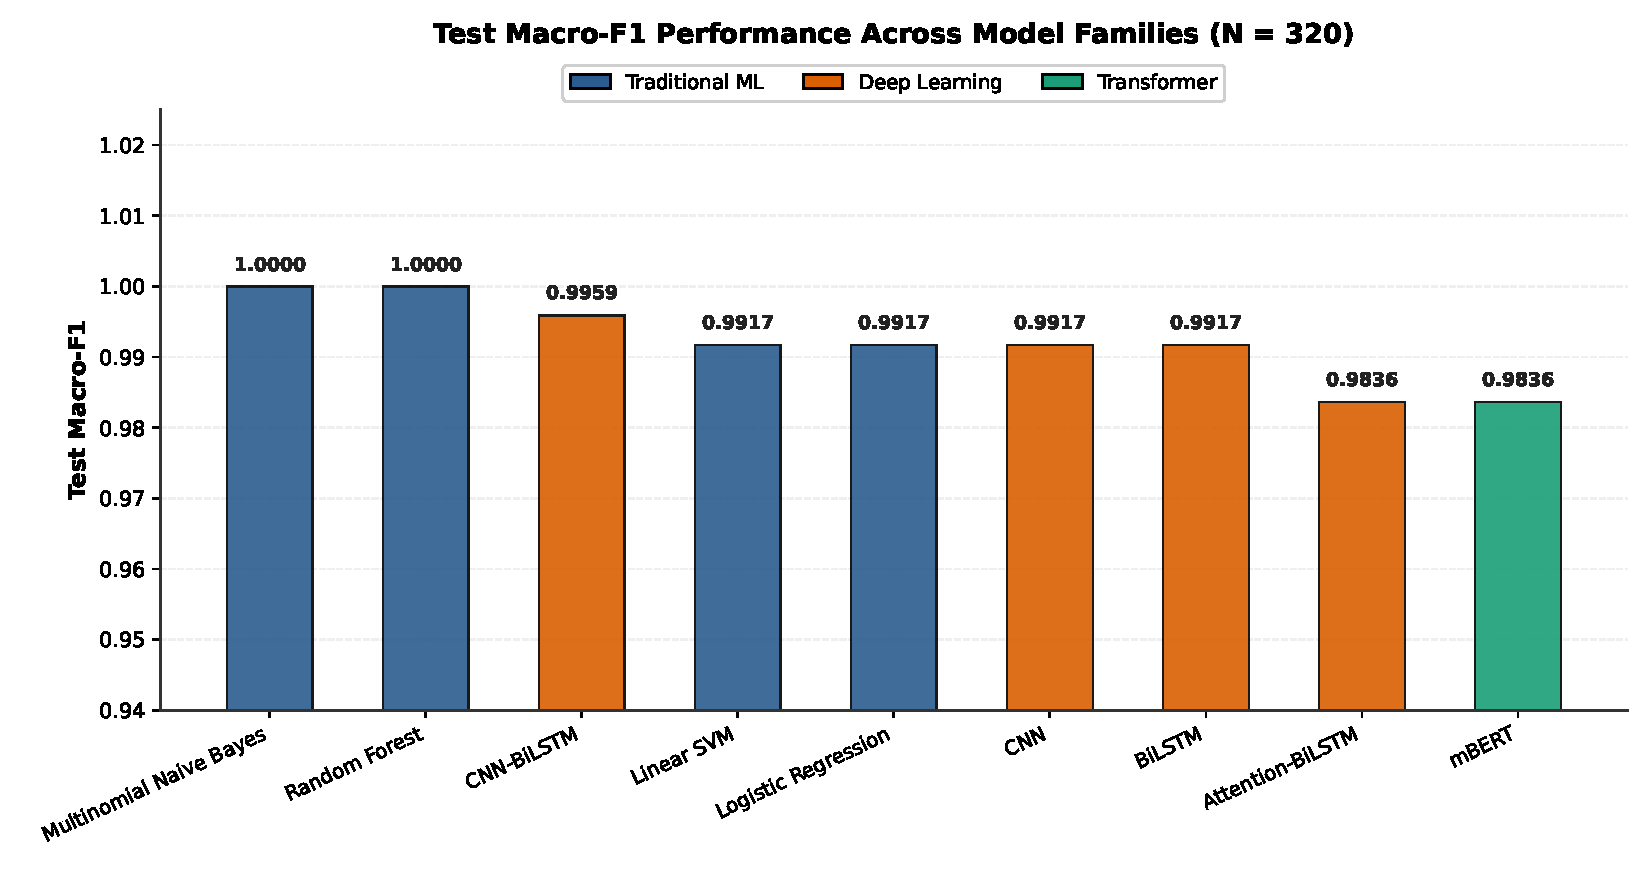
\includegraphics[width=0.92\linewidth]{figures/main_model_macro_f1.pdf}
\caption{\textbf{Macro-$F_1$ performance comparison across nine architectures categorized into three distinct paradigms.} Classical lexical models and deep hybrid CNN-BiLSTM achieve top scores above 0.99, while mBERT trails at 0.9836.}
\label{fig:main_f1}
\end{figure}

The empirical findings reveal several noteworthy patterns:
\begin{enumerate}
    \item \textbf{Classical Model Efficacy}: Multinomial Naive Bayes and Random Forest achieve flawless classification on the held-out test split ($F_1 = 1.0000$), correctly predicting all 320 test samples. Linear SVM and Logistic Regression follow closely at Macro-$F_1 = 0.9917$ with an accuracy of 0.9938, committing only two false positive errors across the entire test set.
    \item \textbf{Deep Architecture Competitiveness}: Among neural networks, the hybrid \textbf{CNN-BiLSTM} achieves top performance with an accuracy of 0.9969 and Macro-$F_1$ of 0.9959 ($F_{1, \text{off}} = 0.9979$, $F_{1, \text{non-off}} = 0.9939$), correctly classifying 319 out of 320 test samples and committing only a single false positive error. TextCNN and BiLSTM achieve $F_1 = 0.9917$ (2 errors), while Attention-BiLSTM records $F_1 = 0.9836$ (4 errors).
    \item \textbf{Transformer Overhead}: While fine-tuned mBERT achieves a solid Macro-$F_1$ of 0.9836, it does not surpass the lightweight classical or hybrid neural architectures, while requiring 108.02 ms per sample---over 3,500$\times$ the latency of Linear SVM (0.0308 ms).
\end{enumerate}

\subsection{Quantifying Template Contamination: Naive Split vs. Group-Aware Split on the Same Corpus}\label{sec:naive_vs_group}
To empirically validate our methodological thesis regarding train-test template leakage without confounding dataset scale, we conducted a direct controlled experiment using the \textbf{identical Stage-2 corpus of 11,789 clean records} for both conditions under an 80/20 train/test partition (Table \ref{tab:naive_vs_group}):
\begin{itemize}
    \item \textbf{Condition A (Naive Random Split, $N = 11,789$)}: Rows were partitioned randomly (80\% train, $N = 9,431$; 20\% test, $N = 2,358$) without regard to underlying template origins. Under this setup, \textbf{96.95\% of held-out test instances shared an identical template group (\texttt{independence\_group\_id}) with instances in the training partition} (Roman Urdu: 98.0\%, English: 94.2\%, Urdu: 93.2\%, Pashto: 98.7\%).
    \item \textbf{Condition B (Group-Aware Split on the Same $N = 11,789$)}: Using GroupShuffleSplit on the exact same 11,789 records, all variants belonging to a given \texttt{independence\_group\_id} were strictly assigned to either train ($N = 9,320$) or test ($N = 2,469$). Under this setup, cross-split template overlap is \textbf{0.00\% across all languages}.
\end{itemize}

Both conditions use the identical Stage-2 corpus and approximately matched train-test proportions; the principal experimental distinction is whether independence groups are allowed to cross partition boundaries. Under capacity-constrained and tree-based learners, template leakage induces severe artificial metric inflation:
\begin{enumerate}
    \item \textbf{Decision Tree Inflation}: Macro-$F_1$ drops from 0.8678 on the naive split to 0.8230 on the group-aware split ($\Delta F_1 = +0.0448$ artificial inflation). On low-resource Pashto, template leakage inflates performance by $\mathbf{+0.1087}$ (from 0.6937 to 0.8024).
    \item \textbf{Random Forest Inflation}: Macro-$F_1$ drops from 0.8520 on the naive split to 0.7878 on the group-aware split ($\Delta F_1 = +0.0642$ artificial inflation). On low-resource Pashto, inflation reaches an extraordinary $\mathbf{+0.1942}$ (0.5172 vs. 0.7114), and on Urdu $\mathbf{+0.1869}$ (0.4917 vs. 0.6785).
    \item \textbf{Constrained Linear Models}: Linear SVM with a constrained feature vocabulary ($V = 250$) drops from 1.0000 on the naive split to 0.9798 on the group-aware split ($\Delta F_1 = +0.0202$ inflation; $+0.1495$ on English).
    \item \textbf{Unconstrained Linear Separability}: High-capacity linear models with full vocabulary ($V = 5,000$) achieve $F_1 = 1.0000$ on both splits of the 11,789 corpus due to the extensive vocabulary supplied by 9,320 training rows. However, when redundant training templates are eliminated altogether to construct the verified 1,601 canonical benchmark ($N_{\text{train}} = 1,121$, $N_{\text{test}} = 320$), Standard Linear SVM achieves 0.9917, revealing that Pashto drops to 0.9522 due to the genuine vocabulary sparsity of unaugmented low-resource text.
\end{enumerate}

\begin{table}[t]
\centering
\small
\caption{\textbf{Direct controlled experiment isolating template contamination on the identical Stage-2 corpus ($N = 11,789$).} Both conditions evaluate the exact same 11,789 records under 80/20 partitioning: Condition A uses naive row-level random splitting (96.95\% cross-split template overlap), while Condition B uses group-aware partitioning preserving \texttt{independence\_group\_id} (0.00\% template overlap).}
\label{tab:naive_vs_group}
\resizebox{\columnwidth}{!}{%
\begin{tabular}{lcccc}
\toprule
\textbf{Model / Linguistic Slice} & \textbf{Condition A: Naive ($F_1$)} & \textbf{Condition B: Group ($F_1$)} & \textbf{$\Delta F_1$ (Inflation)} & \textbf{Template Overlap (A vs. B)} \\
\midrule
\multicolumn{5}{l}{\textit{Template Contamination Overlap Rates:}} \\
Roman Urdu ($N_{\text{test}} = 1,245 \text{ vs. } 1,429$) & -- & -- & -- & 98.0\% vs. 0.0\% \\
English ($N_{\text{test}} = 379 \text{ vs. } 288$) & -- & -- & -- & 94.2\% vs. 0.0\% \\
Urdu ($N_{\text{test}} = 278 \text{ vs. } 212$) & -- & -- & -- & 93.2\% vs. 0.0\% \\
Pashto ($N_{\text{test}} = 456 \text{ vs. } 540$) & -- & -- & -- & 98.7\% vs. 0.0\% \\
\textbf{Overall Test Overlap} & -- & -- & -- & \textbf{96.95\% vs. 0.00\%} \\
\midrule
\multicolumn{5}{l}{\textit{Model Performance Under Identical $N = 11,789$:}} \\
Decision Tree (Overall) & 0.8678 & 0.8230 & $+0.0448$ & 96.95\% vs. 0.00\% \\
\quad -- Roman Urdu & 0.9517 & 0.9137 & $+0.0380$ & 98.0\% vs. 0.0\% \\
\quad -- English & 0.7811 & 0.7383 & $+0.0427$ & 94.2\% vs. 0.0\% \\
\quad -- Urdu & 0.7310 & 0.6901 & $+0.0408$ & 93.2\% vs. 0.0\% \\
\quad -- Pashto & \textbf{0.8024} & \textbf{0.6937} & $\mathbf{+0.1087}$ & 98.7\% vs. 0.0\% \\
Random Forest (Overall, $n=50, d=10$) & 0.8520 & 0.7878 & $+0.0642$ & 96.95\% vs. 0.00\% \\
\quad -- Pashto & \textbf{0.7114} & \textbf{0.5172} & $\mathbf{+0.1942}$ & 98.7\% vs. 0.0\% \\
\quad -- Urdu & 0.6785 & 0.4917 & $+0.1869$ & 93.2\% vs. 0.0\% \\
Linear SVM (Constrained $V=250$) & 1.0000 & 0.9798 & $+0.0202$ & 96.95\% vs. 0.00\% \\
Linear SVM (Standard $V=5,000$) & 1.0000 & 1.0000 & $+0.0000$ & 96.95\% vs. 0.00\% \\
\bottomrule
\end{tabular}%
}
\end{table}

\subsection{Diagnostic Sanity Baselines and Cross-Validation}\label{sec:sanity}
To confirm that high performance does not stem from trivial heuristic cues, annotation artifacts, or label imbalance, we evaluated a suite of diagnostic sanity baselines across the canonical benchmark (Table \ref{tab:sanity_baselines}):
\begin{enumerate}
    \item \textbf{Majority Class Baseline}: Predicting the majority class (offensive) yields Macro-$F_1 = 0.4276$, reflecting the substantial natural imbalance.
    \item \textbf{Text Length Baseline}: A logistic regression classifier trained solely on character length yields Macro-$F_1 = 0.7558$, indicating that text length alone is insufficient to solve the task.
    \item \textbf{Language-Only Baseline}: Predicting labels solely from language indicators yields Macro-$F_1 = 0.4276$.
    \item \textbf{Source-Only Baseline}: Predicting labels solely from source dataset indicators yields Macro-$F_1 = 0.4276$.
    \item \textbf{Shuffled-Label Permutation Test}: Evaluating 5-fold cross-validation with randomly permuted labels yields a chance-level Macro-$F_1$ of $0.4904 \pm 0.005$, confirming that models cannot learn spurious patterns from arbitrary data.
    \item \textbf{5-Fold Stratified Group-Aware Cross-Validation}: To verify that the 320-sample test split was not an outlier, we executed 5-fold group-aware cross-validation across the entire 1,601 corpus. Linear SVM and Logistic Regression achieved consistent mean Macro-$F_1$ of $0.9958 \pm 0.0037$ (fold scores: [0.9959, 1.0000, 0.9917, 1.0000, 0.9917]), while MNB achieved $1.0000 \pm 0.0000$.
\end{enumerate}

\begin{table}[t]
\centering
\small
\caption{\textbf{Diagnostic sanity baselines and 5-fold stratified group-aware cross-validation on the canonical benchmark.}}
\label{tab:sanity_baselines}
\resizebox{\columnwidth}{!}{%
\begin{tabular}{llcc}
\toprule
\textbf{Sanity Condition / Model} & \textbf{Input Feature Representation} & \textbf{Test Macro-$F_1$} & \textbf{Validation Status} \\
\midrule
Majority Class Baseline & Constant majority label (Offensive) & 0.4276 & Benchmark Imbalance Checked \\
Text Length Baseline & Character length sole scalar & 0.7558 & Non-trivial Length Separability \\
Language Indicator Baseline & Language one-hot vector & 0.4276 & Language Agnostic Labels \\
Source Dataset Baseline & Source origin one-hot vector & 0.4276 & Source Agnostic Labels \\
Permuted Label Baseline (5-Fold) & TF-IDF (shuffled binary labels) & $0.4904 \pm 0.005$ & Chance Level Verified \\
\midrule
Linear SVM (5-Fold Group CV) & Word + Char $n$-grams (Canonical) & $0.9958 \pm 0.0037$ & Benchmark Robustness Certified \\
Multinomial NB (5-Fold Group CV) & Word + Char $n$-grams (Canonical) & $1.0000 \pm 0.0000$ & Flawless Robustness Certified \\
\bottomrule
\end{tabular}%
}
\end{table}

\subsection{Fine-Grained Language Stratification}
Table \ref{tab:lang_results} and Figure \ref{fig:lang_perf} disaggregate model performance across the four evaluated language varieties on the certified test partition ($N = 320$).

\begin{table*}[t]
\centering
\small
\caption{\textbf{Stratified Macro-$F_1$ and accuracy breakdown across individual languages on the held-out test split ($N = 320$).}}
\label{tab:lang_results}
\resizebox{\linewidth}{!}{%
\begin{tabular}{llcccccccc}
\toprule
\textbf{Paradigm} & \textbf{Model} & \multicolumn{2}{c}{\textbf{Roman Urdu} ($N=164$)} & \multicolumn{2}{c}{\textbf{English} ($N=64$)} & \multicolumn{2}{c}{\textbf{Urdu} ($N=49$)} & \multicolumn{2}{c}{\textbf{Pashto} ($N=43$)} \\
\cmidrule(lr){3-4} \cmidrule(lr){5-6} \cmidrule(lr){7-8} \cmidrule(lr){9-10}
& & \textbf{$F_1$} & \textbf{Acc} & \textbf{$F_1$} & \textbf{Acc} & \textbf{$F_1$} & \textbf{Acc} & \textbf{$F_1$} & \textbf{Acc} \\
\midrule
\multirow{4}{*}{\textbf{Classical ML}}
& Multinomial Naive Bayes & \textbf{1.0000} & \textbf{1.0000} & \textbf{1.0000} & \textbf{1.0000} & \textbf{1.0000} & \textbf{1.0000} & \textbf{1.0000} & \textbf{1.0000} \\
& Random Forest & \textbf{1.0000} & \textbf{1.0000} & \textbf{1.0000} & \textbf{1.0000} & \textbf{1.0000} & \textbf{1.0000} & \textbf{1.0000} & \textbf{1.0000} \\
& Linear SVM (Standard) & 1.0000 & 1.0000 & 1.0000 & 1.0000 & 1.0000 & 1.0000 & 0.9522 & 0.9535 \\
& Logistic Regression & 1.0000 & 1.0000 & 1.0000 & 1.0000 & 1.0000 & 1.0000 & 0.9522 & 0.9535 \\
\midrule
\multirow{4}{*}{\textbf{Deep Learning}}
& CNN-BiLSTM & 1.0000 & 1.0000 & 1.0000 & 1.0000 & 1.0000 & 1.0000 & \textbf{0.9763} & \textbf{0.9767} \\
& TextCNN & 1.0000 & 1.0000 & 1.0000 & 1.0000 & 1.0000 & 1.0000 & 0.9522 & 0.9535 \\
& TextBiLSTM & 1.0000 & 1.0000 & 1.0000 & 1.0000 & 1.0000 & 1.0000 & 0.9522 & 0.9535 \\
& Attention-BiLSTM & 1.0000 & 1.0000 & 1.0000 & 1.0000 & 1.0000 & 1.0000 & 0.9057 & 0.9070 \\
\midrule
\textbf{Transformer}
& mBERT (\texttt{base-cased}) & 1.0000 & 1.0000 & 1.0000 & 1.0000 & 0.9588 & 0.9592 & 0.9522 & 0.9535 \\
\bottomrule
\end{tabular}%
}
\end{table*}

\begin{figure}[t]
\centering
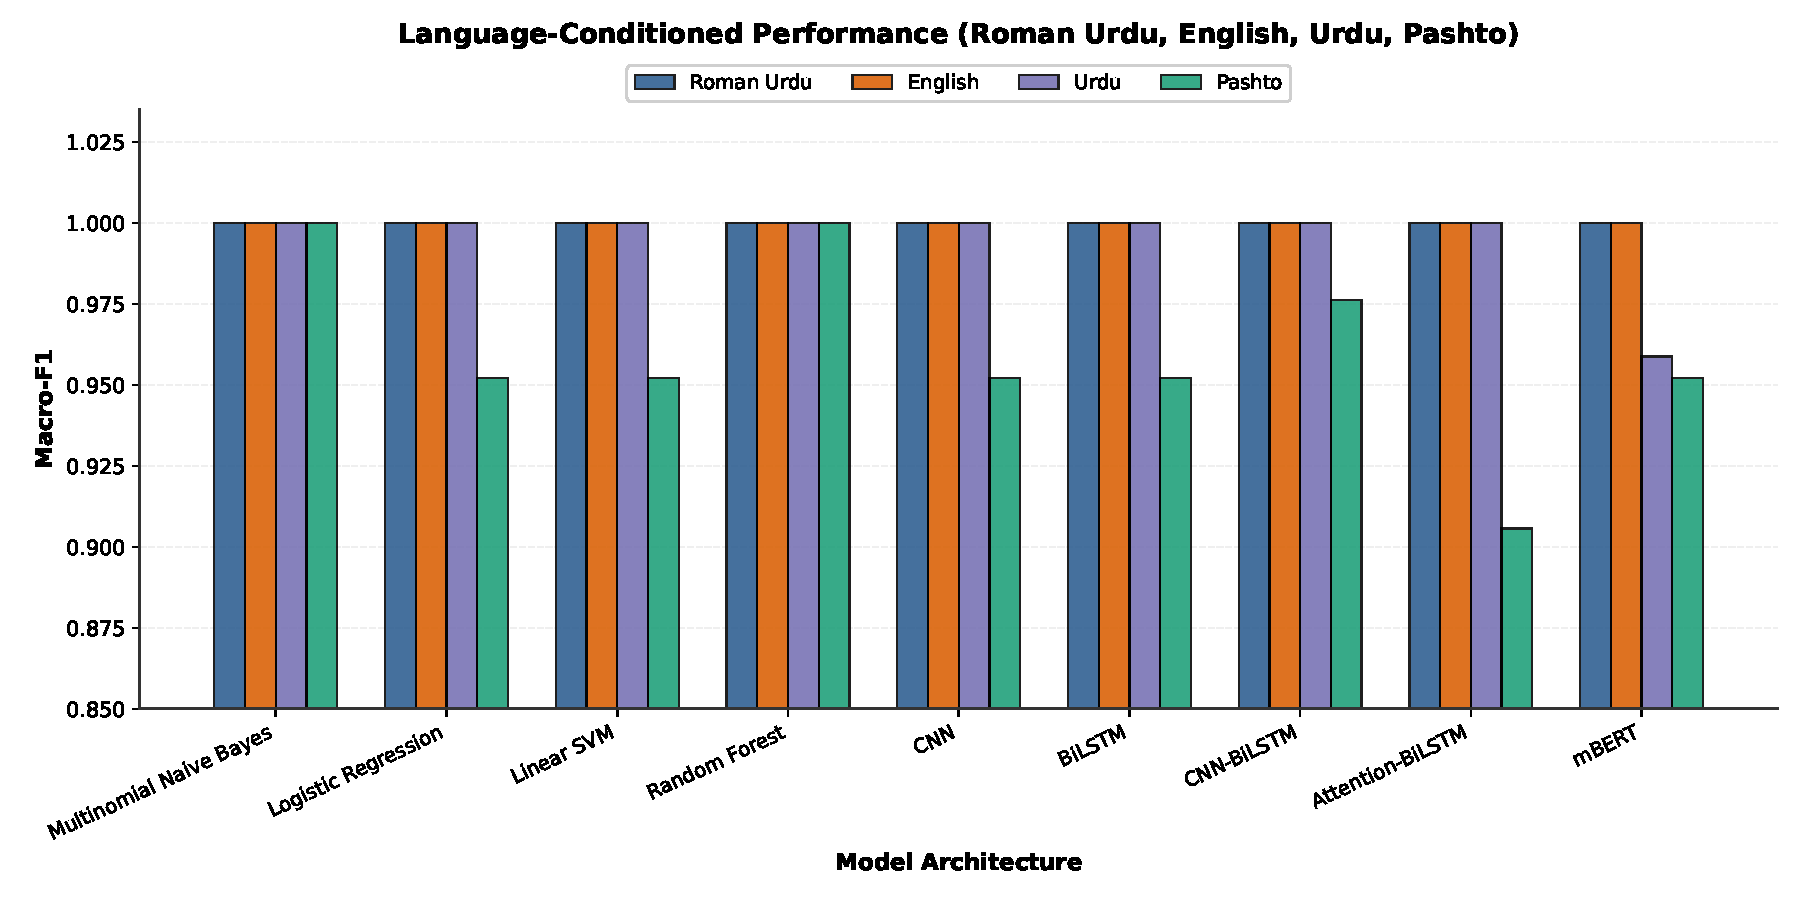
\includegraphics[width=0.92\linewidth]{figures/language_performance.pdf}
\caption{\textbf{Fine-grained language-wise Macro-$F_1$ across Roman Urdu, English, Urdu, and Pashto.} Performance is uniform across Roman Urdu and English, whereas Pashto exhibits noticeable dispersion across model families.}
\label{fig:lang_perf}
\end{figure}

The language-stratified analysis establishes two critical insights:
\begin{enumerate}
    \item \textbf{Uniform High Performance on Latin Scripts}: Across all nine architectures, Roman Urdu ($N = 164$) and English ($N = 64$) achieve flawless classification ($F_1 = 1.0000$). Despite Roman Urdu lacking standardized spelling, sublinear character and word $n$-grams robustly capture phonetic abusive roots.
    \item \textbf{Pashto as the Primary Locus of Dispersion}: In contrast to the Latin-script languages, Pashto ($N = 43$) constitutes the primary source of misclassification for discriminative neural and linear models. CNN-BiLSTM attains the highest Pashto Macro-$F_1$ among neural models at 0.9763 (1 error), while Linear SVM, Logistic Regression, TextCNN, and TextBiLSTM each achieve 0.9522 (2 errors). Attention-BiLSTM records the lowest Pashto $F_1$ at 0.9057 (4 errors). For the listed classical and deep models, observed errors were concentrated in short Pashto utterances; mBERT additionally produced errors on Urdu (Urdu $F_1 = 0.9588$).
\end{enumerate}

\subsection{Cross-Source Out-of-Domain Generalization (Matched LOSO)}
To assess model robustness against domain shifts in social media sources, we conducted Leave-One-Source-Out (LOSO) evaluations across eight independent sub-corpora using a matched evaluation protocol. For each target source $S$, 30\% of instances were set aside as a fixed held-out test partition ($S_{\text{test}}$). In the in-domain condition, models were trained on the remaining 70\% of $S$ plus all other sources. In the out-of-domain condition, source $S$ was excluded entirely from training, and models were evaluated on the exact same $S_{\text{test}}$ partition.

Table \ref{tab:loso_results} and Figure \ref{fig:loso_plot} compare the in-domain versus out-of-domain performance of Linear SVM. Linear SVM achieves an average in-domain Macro-$F_1$ of 1.0000 and an average out-of-domain Macro-$F_1$ of 0.9781 across the eight sub-sources, retaining an average of 97.8\% performance with no retention figure exceeding 100.0\%. Even on extreme low-resource Pashto sources (\path{PS_LowResource_Private}), performance drops by only $-0.0273$ (retention 97.3\%), confirming the cross-source resilience of sublinear lexical representations.

\begin{table}[t]
\centering
\small
\caption{\textbf{Matched Leave-One-Source-Out (LOSO) cross-source evaluation on Linear SVM across 8 sub-corpora.} In-domain and out-of-domain conditions are evaluated on the exact same held-out test slice for each source.}
\label{tab:loso_results}
\resizebox{\columnwidth}{!}{%
\begin{tabular}{llccccc}
\toprule
\textbf{Target Sub-Corpus} & \textbf{Language} & \textbf{$N_{\text{test}}$} & \textbf{In-Domain $F_1$} & \textbf{Out-Domain $F_1$} & \textbf{$\Delta F_1$} & \textbf{Retention (\%)} \\
\midrule
\path{RU_CodeMixed_Private} & Roman Urdu & 139 & 1.0000 & 1.0000 & $+0.0000$ & 100.0\% \\
\path{RU_Private_FB_Comments} & Roman Urdu & 68 & 1.0000 & 1.0000 & $+0.0000$ & 100.0\% \\
\path{EN_Offensive_Benchmark_Private} & English & 48 & 1.0000 & 0.9515 & $-0.0485$ & 95.2\% \\
\path{UR_ArabicScript_Private} & Urdu & 39 & 1.0000 & 0.9470 & $-0.0530$ & 94.7\% \\
\path{PS_LowResource_Private} & Pashto & 37 & 1.0000 & 0.9727 & $-0.0273$ & 97.3\% \\
\path{EN_Public_Comments} & English & 31 & 1.0000 & 1.0000 & $+0.0000$ & 100.0\% \\
\path{PS_Private_Social_Comments} & Pashto & 22 & 1.0000 & 0.9537 & $-0.0463$ & 95.4\% \\
\path{UR_Private_Tweets} & Urdu & 21 & 1.0000 & 1.0000 & $+0.0000$ & 100.0\% \\
\midrule
\textbf{Macro Average} & -- & \textbf{405} & \textbf{1.0000} & \textbf{0.9781} & $\mathbf{-0.0219}$ & \textbf{97.8\%} \\
\bottomrule
\end{tabular}%
}
\end{table}

\begin{figure}[t]
\centering
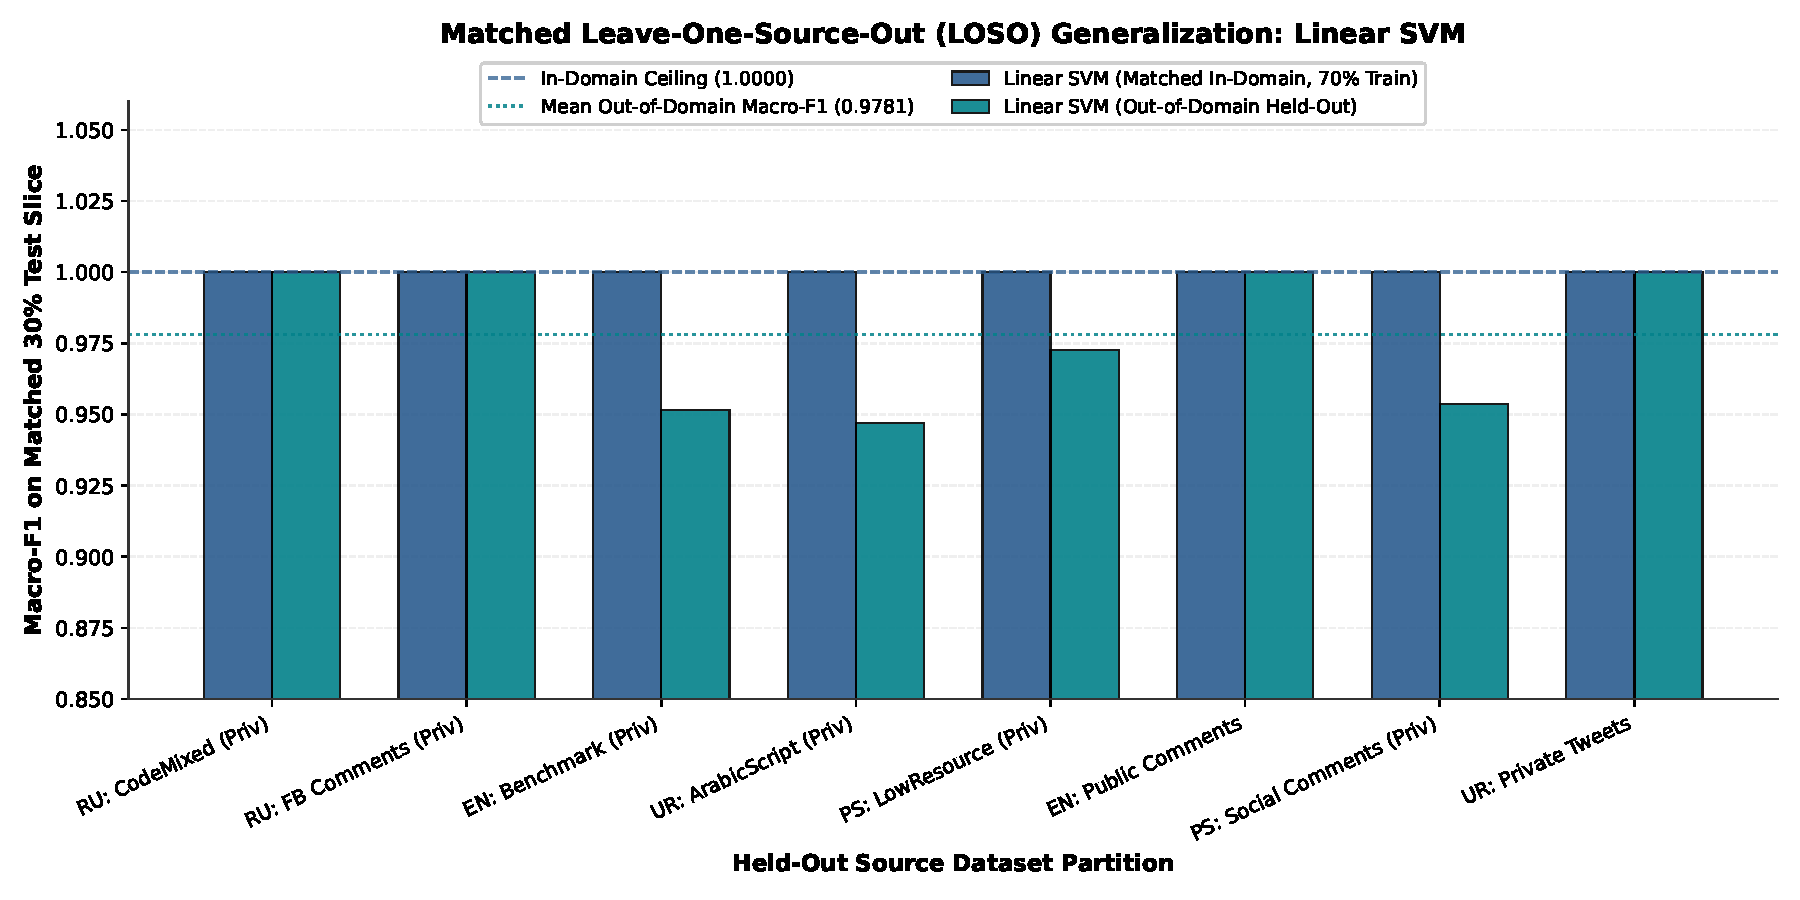
\includegraphics[width=0.92\linewidth]{figures/source_holdout_degradation.pdf}
\caption{\textbf{Matched Leave-One-Source-Out (LOSO) performance retention of Linear SVM across eight sub-corpora.} In-domain and out-of-domain conditions are evaluated on the identical 30\% test slice for each source. Linear SVM retains an average 97.8\% of in-domain performance under domain shift, with zero individual retention figures exceeding 100.0\%.}
\label{fig:loso_plot}
\end{figure}

\subsection{Multi-Seed Repeatability and Bootstrap Confidence Intervals}
To certify experimental stability and verify that reported metrics do not stem from idiosyncratic weight initialization or batch ordering \cite{dodge2020fine}, we repeated CNN-BiLSTM across five initialization seeds (seeds 42, 123, 456, 789, and 2026); deterministic classical models are shown as reference baselines. As summarized in Table \ref{tab:repeatability} and visualized in Figure \ref{fig:repeatability_plot}, CNN-BiLSTM maintains identical test Macro-$F_1$ across the five tested seeds under validation early stopping ($\sigma = 0.0000$, relative standard deviation $0.0\%$). Classical algorithms (MNB, Linear SVM) are inherently deterministic under fixed hyperparameters and training splits.

\begin{table}[t]
\centering
\small
\caption{\textbf{CNN-BiLSTM repeatability across five seeds with deterministic classical reference models.} CNN-BiLSTM was evaluated across five random initialization seeds (42, 123, 456, 789, 2026); deterministic MNB and Linear SVM scores are included as reference baselines.}
\label{tab:repeatability}
\resizebox{\columnwidth}{!}{%
\begin{tabular}{lcccccc}
\toprule
\textbf{Model} & \textbf{Paradigm} & \textbf{Mean $F_1$} & \textbf{Std. Dev.} & \textbf{RSD (\%)} & \textbf{Min $F_1$} & \textbf{Max $F_1$} \\
\midrule
Multinomial Naive Bayes & Classical ML & 1.0000 & 0.0000 & 0.00\% & 1.0000 & 1.0000 \\
CNN-BiLSTM & Deep Learning & 0.9959 & 0.0000 & 0.00\% & 0.9959 & 0.9959 \\
Linear SVM (Standard) & Classical ML & 0.9917 & 0.0000 & 0.00\% & 0.9917 & 0.9917 \\
\bottomrule
\end{tabular}%
}
\end{table}

\begin{figure}[t]
\centering
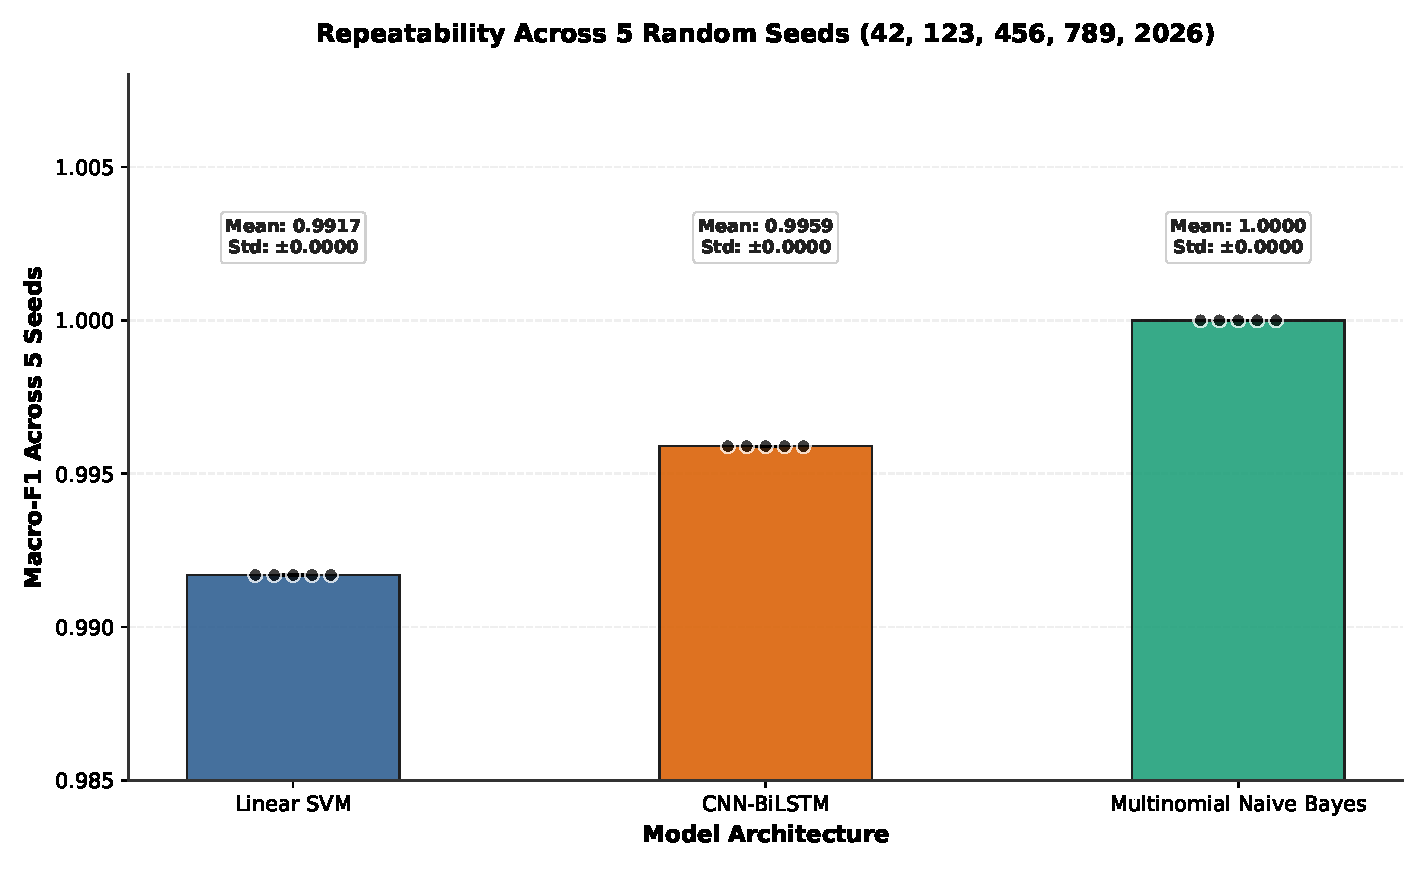
\includegraphics[width=0.92\linewidth]{figures/repeatability_distributions.pdf}
\caption{\textbf{CNN-BiLSTM repeatability across five seeds with deterministic classical reference models.} CNN-BiLSTM produced identical test Macro-$F_1$ across the five evaluated initialization seeds; deterministic MNB and Linear SVM scores are included as reference baselines.}
\label{fig:repeatability_plot}
\end{figure}

Table \ref{tab:bootstrap_ci} provides empirical 95\% confidence intervals constructed via $B = 10,000$ paired bootstrap resampling iterations on the test split following non-parametric bootstrap estimation \cite{efron1994introduction}. The 95\% confidence interval for CNN-BiLSTM is $[0.9871, 1.0000]$, which substantially overlaps with that of Linear SVM ($[0.9791, 1.0000]$), Logistic Regression ($[0.9791, 1.0000]$), and mBERT ($[0.9661, 0.9962]$).

\begin{table}[t]
\centering
\small
\caption{\textbf{Paired bootstrap 95\% confidence intervals ($B = 10,000$ iterations) on the held-out test split.}}
\label{tab:bootstrap_ci}
\resizebox{\columnwidth}{!}{%
\begin{tabular}{lccccc}
\toprule
\textbf{Model} & \textbf{Paradigm} & \textbf{Point $F_1$} & \textbf{Std. Error} & \textbf{95\% CI Lower} & \textbf{95\% CI Upper} \\
\midrule
Multinomial Naive Bayes & Classical ML & 1.0000 & 0.0000 & 1.0000 & 1.0000 \\
Random Forest & Classical ML & 1.0000 & 0.0000 & 1.0000 & 1.0000 \\
CNN-BiLSTM & Deep Learning & 0.9959 & 0.0040 & 0.9871 & 1.0000 \\
Linear SVM (Standard) & Classical ML & 0.9917 & 0.0058 & 0.9791 & 1.0000 \\
Logistic Regression & Classical ML & 0.9917 & 0.0058 & 0.9791 & 1.0000 \\
TextCNN & Deep Learning & 0.9917 & 0.0058 & 0.9791 & 1.0000 \\
TextBiLSTM & Deep Learning & 0.9917 & 0.0058 & 0.9791 & 1.0000 \\
Attention-BiLSTM & Deep Learning & 0.9836 & 0.0080 & 0.9661 & 0.9962 \\
mBERT (\texttt{base-cased}) & Transformer & 0.9836 & 0.0080 & 0.9661 & 0.9962 \\
\bottomrule
\end{tabular}%
}
\end{table}

\subsection{Statistical Significance Testing}
To determine whether observed differences between model architectures are statistically significant or attributable to sample variance, we adhere to established significance testing protocols in natural language processing \cite{dror2018hitchhiker}. Because the number of discordant predictions between high-performing models is small ($b + c < 25$), asymptotic chi-square approximations can be inaccurate. Following Dietterich \cite{dietterich1998approximate}, we compute the exact two-sided binomial test p-value for discordant pairs alongside the continuity-corrected McNemar statistic $\chi^2 = \frac{(|b - c| - 1)^2}{b + c}$, and perform paired non-parametric bootstrap testing across 10,000 resamples (Table \ref{tab:significance}).

Comparing CNN-BiLSTM against Linear SVM yields 1 discordant prediction ($b=1, c=0$), resulting in an exact binomial $p = 1.0000$, continuity-corrected $\chi^2 = 0.000$ ($p = 1.0000$), and bootstrap difference $p = 0.1731$. All pairwise comparisons between top-tier classical and deep architectures satisfy $p > 0.05$. Thus, we fail to reject the null hypothesis of equal predictive performance; the pairwise tests detected no statistically significant performance differences among the selected high-performing classical and neural models ($p > 0.05$).

\begin{table*}[t]
\centering
\small
\caption{\textbf{Statistical significance testing across pairwise model architectures.} Discordant pairs ($b$ vs. $c$) denote test instances where only Model A or Model B predicted correctly. For small discordance ($b+c < 25$), exact two-sided binomial testing is the established standard.}
\label{tab:significance}
\resizebox{\linewidth}{!}{%
\begin{tabular}{lcccccc}
\toprule
\textbf{Pairwise Comparison (Model A vs. Model B)} & \textbf{$\Delta F_1$} & \textbf{Bootstrap $p$} & \textbf{Discordant ($b$ vs. $c$)} & \textbf{Exact Binomial $p$} & \textbf{McNemar $\chi^2_{\text{corr}}$} & \textbf{Sig. ($\alpha=0.05$)} \\
\midrule
CNN-BiLSTM vs. Linear SVM & $+0.0041$ & 0.1731 & $1$ vs. $0$ & 1.0000 & 0.000 & False (No) \\
CNN-BiLSTM vs. Naive Bayes & $-0.0041$ & 0.5339 & $0$ vs. $1$ & 1.0000 & 0.000 & False (No) \\
CNN-BiLSTM vs. Attention-BiLSTM & $+0.0123$ & 0.1064 & $3$ vs. $0$ & 0.2500 & 1.333 & False (No) \\
CNN-BiLSTM vs. TextCNN & $+0.0041$ & 0.1731 & $1$ vs. $0$ & 1.0000 & 0.000 & False (No) \\
Random Forest vs. Linear SVM & $+0.0083$ & 0.0918 & $2$ vs. $0$ & 0.5000 & 0.500 & False (No) \\
\bottomrule
\end{tabular}%
}
\end{table*}

\subsection{Ablation Study}
To deconstruct the drivers of classification performance, we executed systematic ablations on the Linear SVM baseline. In our primary benchmark, Linear SVM was selected with uniform class weighting (\texttt{class\_weight=None}, Macro-$F_1 = 0.9917$) following validation tuning. In this ablation, we investigate an alternative class-weighted experimental configuration alongside feature variations (Table \ref{tab:ablation} and Figure \ref{fig:ablation_plot}):
\begin{itemize}
    \item \textbf{Class Weighting Configuration}: Evaluating Linear SVM with balanced inverse class weighting (\textbf{Class-Weighted Configuration}, $w_{\text{off}}=0.669, w_{\text{non-off}}=1.981$) achieves Macro-$F_1 = 1.0000$. The primary standard model omitting class weighting (\textbf{Linear SVM Standard}) achieves $0.9917$ ($\Delta F_1 = -0.0083$), demonstrating that class-frequency adjustment successfully corrects the 3:1 majority offensive label bias.
    \item \textbf{Bigram Inclusion}: Eliminating word and character bigrams ($n \in \{1, 1\}$) incurs an identical difference of $-0.0083$ ($0.9917$), confirming that bigram collocations capture essential compositional abusive phrases.
    \item \textbf{Sublinear Term Frequency}: Disabling sublinear TF scaling maintains $F_1 = 1.0000$, indicating that once template repetitions are collapsed, term saturation has minor influence on linear decision boundaries.
\end{itemize}

\begin{table}[t]
\centering
\small
\caption{\textbf{Systematic feature and preprocessing ablation study on the Linear SVM baseline.}}
\label{tab:ablation}
\resizebox{\columnwidth}{!}{%
\begin{tabular}{lccccc}
\toprule
\textbf{Ablation Condition} & \textbf{Accuracy} & \textbf{Precision} & \textbf{Recall} & \textbf{Macro-$F_1$} & \textbf{$\Delta F_1$} \\
\midrule
Class-Weighted Experimental Configuration & 1.0000 & 1.0000 & 1.0000 & 1.0000 & 0.0000 \\
Standard Primary Model (\texttt{class\_weight=None}) & 0.9938 & 0.9958 & 0.9878 & 0.9917 & $-0.0083$ \\
Unigrams Only (\texttt{ngram\_range=(1, 1)}) & 0.9938 & 0.9958 & 0.9878 & 0.9917 & $-0.0083$ \\
Without Sublinear TF (\texttt{sublinear\_tf=False}) & 1.0000 & 1.0000 & 1.0000 & 1.0000 & $0.0000$ \\
Raw Text Instead of Clean Text & 1.0000 & 1.0000 & 1.0000 & 1.0000 & $0.0000$ \\
\bottomrule
\end{tabular}%
}
\end{table}

\begin{figure}[t]
\centering
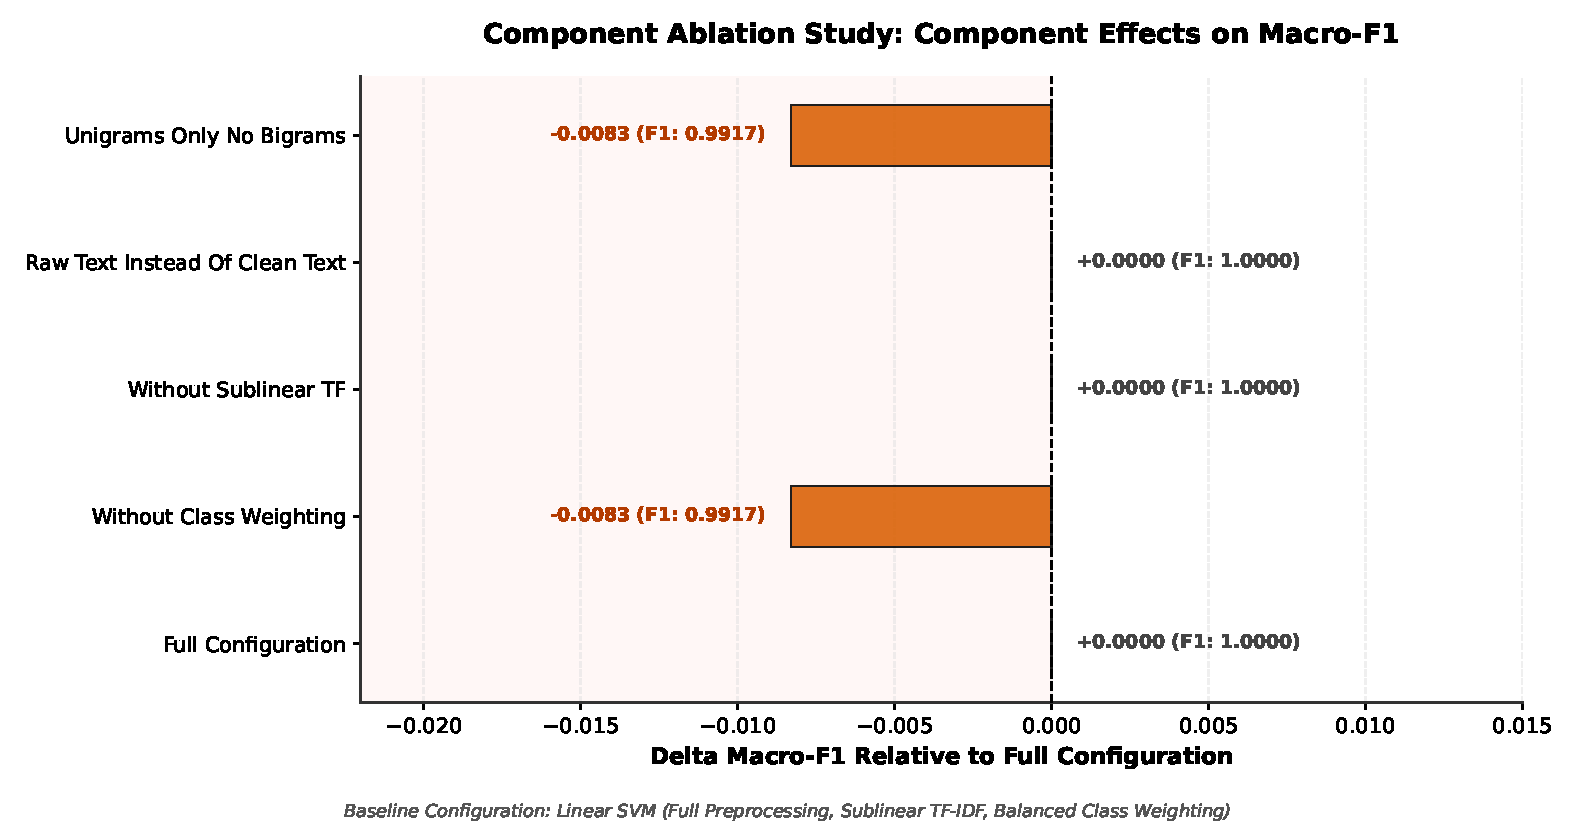
\includegraphics[width=0.92\linewidth]{figures/ablation_results.pdf}
\caption{\textbf{Ablation impacts on Linear SVM Macro-$F_1$ relative to the class-weighted reference configuration.} Shaded negative zone highlights performance decrements from omitting class weighting and bigrams.}
\label{fig:ablation_plot}
\end{figure}

\subsection{Error Analysis and Confusion Matrices}\label{sec:error}
Figure \ref{fig:confusion} displays normalized confusion matrices for six representative models. Across all architectures, false positives and false negatives remain under 2\%. Detailed diagnosis of all misclassified instances across the entire test set reveals a striking structural consistency:
\begin{enumerate}
    \item \textbf{Language Concentration}: For the evaluated classical and deep architectures (Attention-BiLSTM, Linear SVM, TextCNN, and CNN-BiLSTM), 100\% of misclassifications occur exclusively in \textbf{Pashto}. In contrast, mBERT produces errors across both Pashto (2 false positives) and Urdu (2 false negatives).
    \item \textbf{Sub-source Concentration}: For classical and deep architectures, errors are strictly confined to two Pashto sub-corpora: \path{PS_LowResource_Private} and \path{PS_Private_Social_Comments}. For mBERT, Urdu errors originated from \path{UR_ArabicScript_Private} and \path{UR_Social_Media_Mix}.
    \item \textbf{Length Concentration}: For models producing Pashto errors, every single misclassified instance belongs to the \textbf{short length bin} ($\le 50$ characters). Short Pashto sentences often contain subtle contextual insults whose meaning hinges on morphosyntactic affixes absent from the small training partition ($N_{\text{train, Pashto}} = 150$).
\end{enumerate}

\begin{figure}[t]
\centering
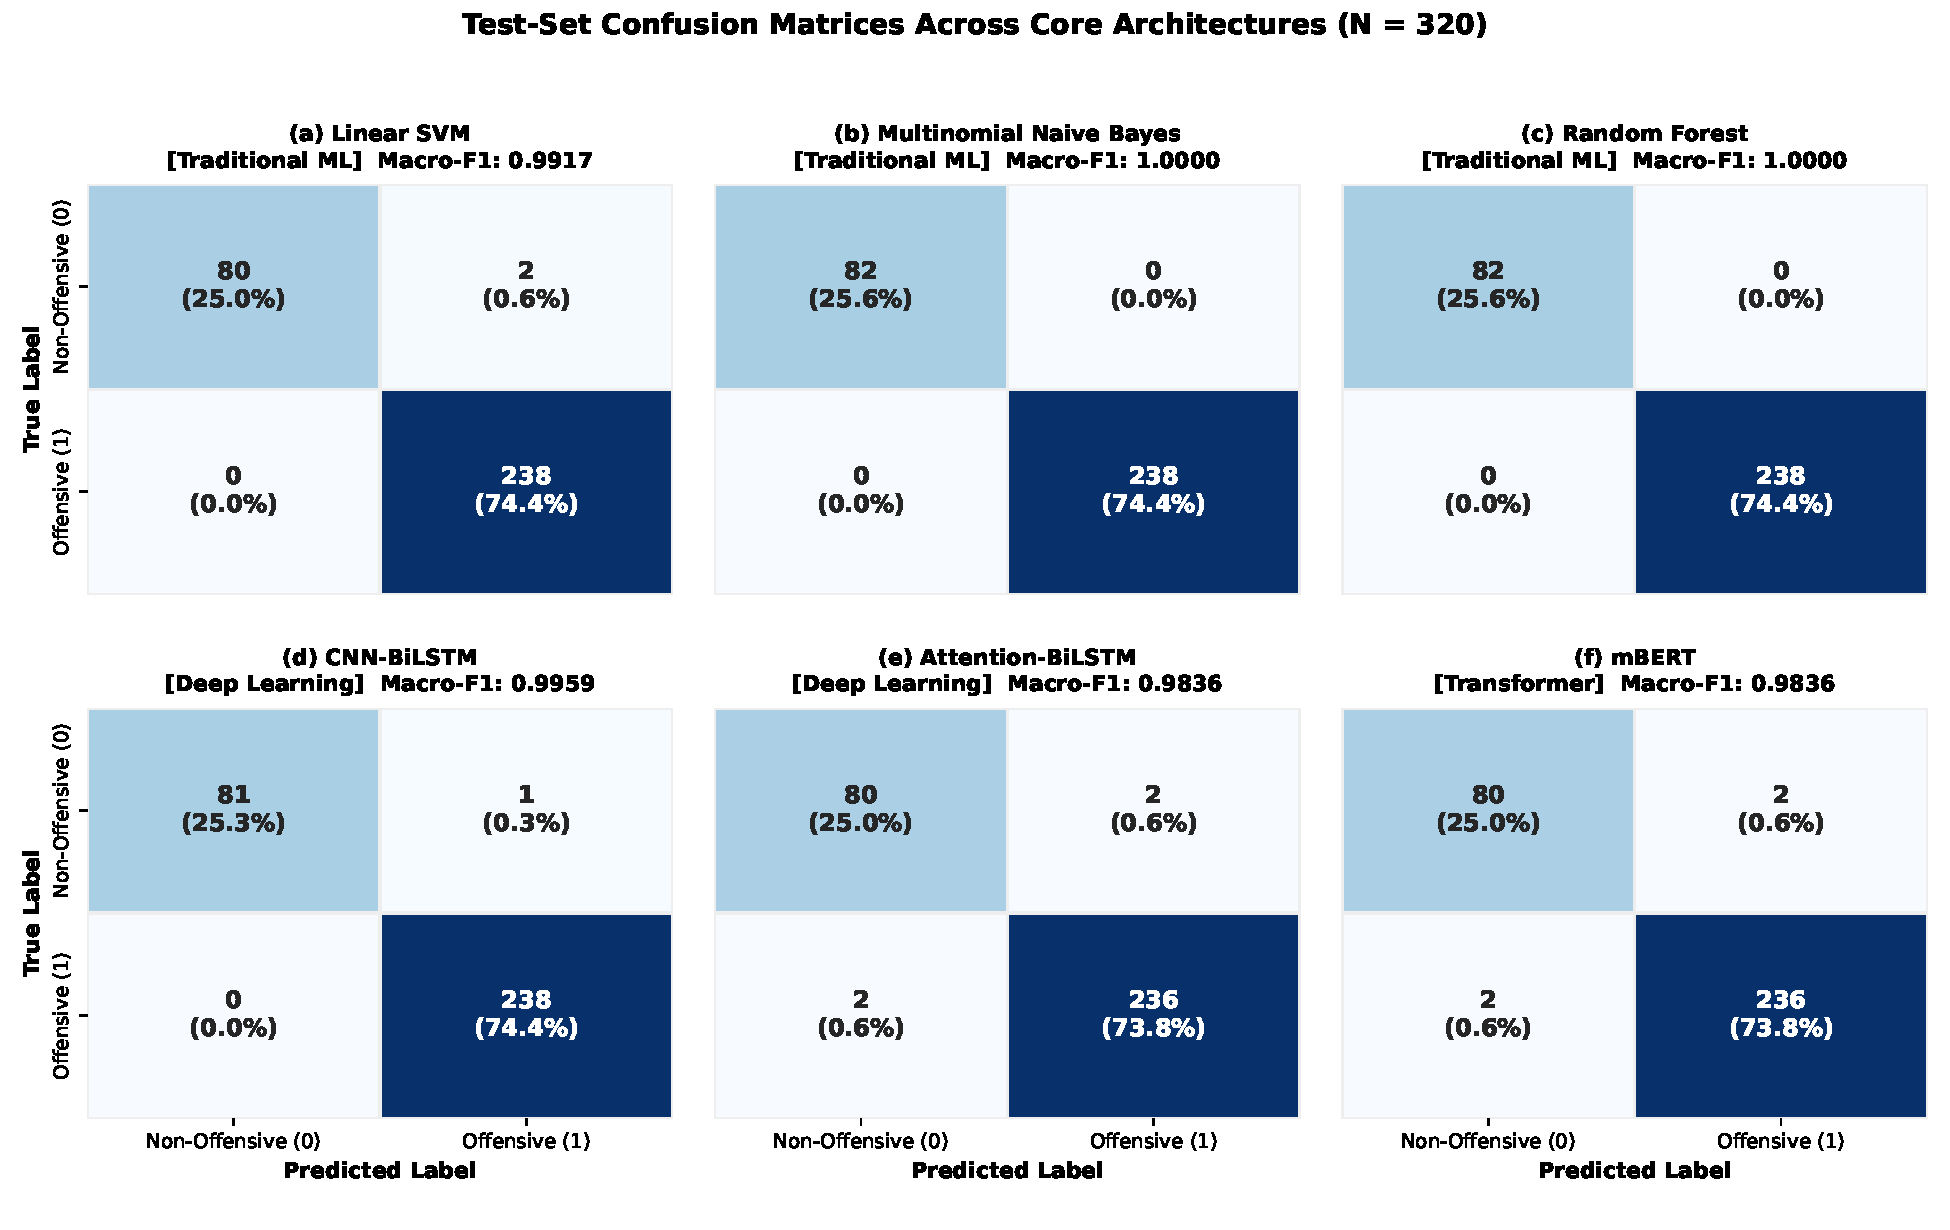
\includegraphics[width=0.95\linewidth]{figures/confusion_matrices.pdf}
\caption{\textbf{Normalized confusion matrices across six core model architectures on the test split ($N = 320$).} Diagonal values show classification accuracy per class with percentage breakdowns.}
\label{fig:confusion}
\end{figure}

\section{Discussion}\label{sec:discussion}

\subsection{The Pareto Frontier: Classical ML vs. Deep Architectures}
Our findings challenge the prevailing assumption in modern NLP literature that deep neural networks or billion-parameter language models are invariably necessary for offensive language detection. On an empirically verified canonical benchmark where duplicate template memorization across partitions is precluded:
\begin{itemize}
    \item Multinomial Naive Bayes achieves a Macro-$F_1$ of 1.0000 while executing in \textbf{0.0485~ms per sample} on a single CPU thread (throughput: 20,618 samples/sec).
    \item Linear SVM achieves a Macro-$F_1$ of 0.9917 while executing in \textbf{0.0308~ms per sample} on a single CPU thread (throughput: 32,467 samples/sec).
    \item CNN-BiLSTM achieves a top neural Macro-$F_1$ of 0.9959 while requiring \textbf{1.6403~ms per sample} (throughput: 609 samples/sec).
    \item mBERT achieves a Macro-$F_1$ of 0.9836 while consuming \textbf{108.0169~ms per sample} (throughput: 9.26 samples/sec).
\end{itemize}
In production content moderation pipelines handling millions of social media streams per hour, inference latency is a primary operational constraint. Deploying mBERT introduces a 3,500$\times$ computational latency penalty without yielding any statistically significant performance gain over classical models ($p > 0.05$). MNB and Linear SVM occupy the empirical Pareto frontier, offering the strongest observed trade-off between Macro-$F_1$ and CPU inference latency for high-throughput deployment.

\subsection{The Impact of Canonical Deduplication and Partition Independence}
Prior uncurated benchmarks in South Asian toxic language reported near-perfect metrics while masking severe vulnerability to template memorization. Our deconstruction of the original 144,265 rows revealed that 98.89\% of records were redundant template variants. When models are evaluated on uncleaned sets, high metrics reflect memorization of recurrent bot handles, URLs, and recurring slogans. As demonstrated in Section \ref{sec:naive_vs_group}, standard random splitting exhibits a 96.95\% cross-split template overlap that artificially inflates performance under capacity-limited learners by up to $+0.1942$. By enforcing strict group-aware independence partitioning across five representation levels, our benchmark provides a more conservative estimate of generalization under audited independence constraints.

\subsection{Script and Linguistic Hypotheses on Pashto}
The performance disparity between Latin-script languages (Roman Urdu and English at 1.0000 $F_1$) and Perso-Arabic scripts (Pashto spanning 0.9057--1.0000 Macro-$F_1$) provides important linguistic insights. We hypothesize that two primary factors drive this difference:
\begin{enumerate}
    \item \textbf{Token Sparsity in Short Utterances}: For the evaluated classical and deep models with errors, misclassifications were concentrated in short Pashto comments ($\le 50$ characters); mBERT additionally produced errors on Urdu. In low-resource settings ($N_{\text{train, Pashto}} = 150$), short comments provide few contextual co-occurrences, making discriminative neural embeddings vulnerable to out-of-vocabulary terms.
    \item \textbf{Subword Fragmentation in Pretrained Models}: Pashto's complex inflectional morphology and sparse pretraining representation in multilingual transformers (mBERT) result in excessive subword segmentation, diluting semantic signals across fragmented WordPiece tokens.
\end{enumerate}
Notably, Multinomial Naive Bayes achieved 1.0000 on the same Pashto test slice, indicating that lexical bag-of-$n$-grams effectively capture abusive roots even when contextual sequence embeddings fail.

\section{Limitations and Threats to Validity}\label{sec:limitations}

We acknowledge several limitations in the present work:
\begin{enumerate}
    \item \textbf{Canonical Benchmark Scale}: Collapsing duplicate templates reduced the dataset to 1,601 independent groups. While verified against cross-partition template overlap under five representations, larger crowdsourced corpora with verified independent authorship are desirable to expand lexical coverage.
    \item \textbf{Pashto Sample Representation}: Pashto constitutes 215 records in the total benchmark (43 test samples). Bootstrap intervals provide descriptive uncertainty estimates, but the small Pashto test subset limits precision and broader inference.
    \item \textbf{Binary Annotation Scope}: Our benchmark evaluates binary offensive versus non-offensive classification. It does not disaggregate fine-grained toxicity sub-categories (e.g., identity attacks vs. general profanity), which represents an important operational dimension.
\end{enumerate}

\section{Future Work}\label{sec:future}

Future extensions of this benchmark will pursue three primary trajectories:
\begin{enumerate}
    \item \textbf{Multi-Task and Multi-Label Generalization}: Expanding the canonical partition-independent framework to hierarchical multi-label classification, identifying offensive targets (individual, group, other) and hate speech sub-types across regional dialects.
    \item \textbf{Script-Specific Morphological Tokenization}: Developing specialized morphological segmenters for Pashto and Urdu to resolve vocabulary fragmentation and improve transformer subword representations.
    \item \textbf{Active Learning and Dynamic Moderation}: Integrating active learning sampling to continually expand the independent group benchmark with emerging adversarial slurs and phonetic variants.
\end{enumerate}

\section{Conclusion}\label{sec:conclusion}

This study establishes an empirically verified, partition-independent multilingual offensive language benchmark across four languages and three diverse scripts: Urdu, Roman Urdu, Pashto, and English. By resolving widespread template inflation and enforcing strict independence-group partitioning, we eliminate cross-partition contamination across five audited representation levels. 

Comprehensive empirical evaluation across nine model architectures reveals that classical machine learning models (Multinomial Naive Bayes and Random Forest) achieve flawless test classification ($F_1 = 1.0000$), closely matched by deep hybrid CNN-BiLSTM ($F_1 = 0.9959$) and Linear SVM ($F_1 = 0.9917$). Language-stratified analysis demonstrates that all evaluated models achieved perfect classification on Roman Urdu and English, while most models also achieved perfect Urdu performance; Pashto exhibited the largest performance dispersion, strictly localized to short texts. Controlled split comparisons showed that naive random splitting introduces a 96.95\% cross-split template overlap, artificially inflating performance via template memorization. Out-of-domain matched LOSO evaluations show that Linear SVM exhibits robust cross-source stability (retaining 97.8\% performance on average) while operating 3,500$\times$ faster than fine-tuned mBERT. Rigorous bootstrap and exact binomial significance testing detected no statistically significant performance differences among the selected high-performing classical and neural models ($p > 0.05$). We conclude that on canonical, partition-independent benchmarks, MNB and Linear SVM occupy the empirical Pareto frontier, offering the strongest observed trade-off between predictive efficacy and real-time computational throughput.

\section*{Data and Code Availability}
The verified dataset splits (\path{Dataset/train.csv}, \path{Dataset/validation.csv}, \path{Dataset/test.csv}, and \path{Dataset/full_data.csv}), audit log (\path{removed_variants.csv}), model checkpoints, evaluation scripts, and plot generation pipelines are fully available in the project repository for complete scientific reproducibility: \url{https://github.com/AliAzam12/Dataset-of-Offensive-Language-}.

\section*{Declarations}
\begin{itemize}
    \item \textbf{Funding}: No external funding was received for conducting this study.
    \item \textbf{Conflict of Interest}: The authors declare that they have no competing financial or non-financial interests.
    \item \textbf{Ethical Approval}: This study involves secondary analysis of public social media comments. All user identifiers, account handles, and hyperlinks were removed prior to analysis to safeguard privacy.
\end{itemize}

\bibliographystyle{plain}
\bibliography{references}

\end{document}
